% Options for packages loaded elsewhere
\PassOptionsToPackage{unicode}{hyperref}
\PassOptionsToPackage{hyphens}{url}
%
\documentclass[
  american,
  man,floatsintext]{apa7}
\usepackage{lmodern}
\usepackage{amssymb,amsmath}
\usepackage{ifxetex,ifluatex}
\ifnum 0\ifxetex 1\fi\ifluatex 1\fi=0 % if pdftex
  \usepackage[T1]{fontenc}
  \usepackage[utf8]{inputenc}
  \usepackage{textcomp} % provide euro and other symbols
\else % if luatex or xetex
  \usepackage{unicode-math}
  \defaultfontfeatures{Scale=MatchLowercase}
  \defaultfontfeatures[\rmfamily]{Ligatures=TeX,Scale=1}
\fi
% Use upquote if available, for straight quotes in verbatim environments
\IfFileExists{upquote.sty}{\usepackage{upquote}}{}
\IfFileExists{microtype.sty}{% use microtype if available
  \usepackage[]{microtype}
  \UseMicrotypeSet[protrusion]{basicmath} % disable protrusion for tt fonts
}{}
\makeatletter
\@ifundefined{KOMAClassName}{% if non-KOMA class
  \IfFileExists{parskip.sty}{%
    \usepackage{parskip}
  }{% else
    \setlength{\parindent}{0pt}
    \setlength{\parskip}{6pt plus 2pt minus 1pt}}
}{% if KOMA class
  \KOMAoptions{parskip=half}}
\makeatother
\usepackage{xcolor}
\IfFileExists{xurl.sty}{\usepackage{xurl}}{} % add URL line breaks if available
\IfFileExists{bookmark.sty}{\usepackage{bookmark}}{\usepackage{hyperref}}
\hypersetup{
  pdftitle={Supplement: Moral Dilution},
  pdfauthor={Cillian McHugh1 \& Eric R. Igou1},
  pdflang={en-US},
  pdfkeywords={keywords},
  hidelinks,
  pdfcreator={LaTeX via pandoc}}
\urlstyle{same} % disable monospaced font for URLs
\usepackage{graphicx,grffile}
\makeatletter
\def\maxwidth{\ifdim\Gin@nat@width>\linewidth\linewidth\else\Gin@nat@width\fi}
\def\maxheight{\ifdim\Gin@nat@height>\textheight\textheight\else\Gin@nat@height\fi}
\makeatother
% Scale images if necessary, so that they will not overflow the page
% margins by default, and it is still possible to overwrite the defaults
% using explicit options in \includegraphics[width, height, ...]{}
\setkeys{Gin}{width=\maxwidth,height=\maxheight,keepaspectratio}
% Set default figure placement to htbp
\makeatletter
\def\fps@figure{htbp}
\makeatother
\setlength{\emergencystretch}{3em} % prevent overfull lines
\providecommand{\tightlist}{%
  \setlength{\itemsep}{0pt}\setlength{\parskip}{0pt}}
\setcounter{secnumdepth}{-\maxdimen} % remove section numbering
% Make \paragraph and \subparagraph free-standing
\ifx\paragraph\undefined\else
  \let\oldparagraph\paragraph
  \renewcommand{\paragraph}[1]{\oldparagraph{#1}\mbox{}}
\fi
\ifx\subparagraph\undefined\else
  \let\oldsubparagraph\subparagraph
  \renewcommand{\subparagraph}[1]{\oldsubparagraph{#1}\mbox{}}
\fi
% Manuscript styling
\usepackage{upgreek}
\captionsetup{font=singlespacing,justification=justified}

% Table formatting
\usepackage{longtable}
\usepackage{lscape}
% \usepackage[counterclockwise]{rotating}   % Landscape page setup for large tables
\usepackage{multirow}		% Table styling
\usepackage{tabularx}		% Control Column width
\usepackage[flushleft]{threeparttable}	% Allows for three part tables with a specified notes section
\usepackage{threeparttablex}            % Lets threeparttable work with longtable

% Create new environments so endfloat can handle them
% \newenvironment{ltable}
%   {\begin{landscape}\centering\begin{threeparttable}}
%   {\end{threeparttable}\end{landscape}}
\newenvironment{lltable}{\begin{landscape}\centering\begin{ThreePartTable}}{\end{ThreePartTable}\end{landscape}}

% Enables adjusting longtable caption width to table width
% Solution found at http://golatex.de/longtable-mit-caption-so-breit-wie-die-tabelle-t15767.html
\makeatletter
\newcommand\LastLTentrywidth{1em}
\newlength\longtablewidth
\setlength{\longtablewidth}{1in}
\newcommand{\getlongtablewidth}{\begingroup \ifcsname LT@\roman{LT@tables}\endcsname \global\longtablewidth=0pt \renewcommand{\LT@entry}[2]{\global\advance\longtablewidth by ##2\relax\gdef\LastLTentrywidth{##2}}\@nameuse{LT@\roman{LT@tables}} \fi \endgroup}

% \setlength{\parindent}{0.5in}
% \setlength{\parskip}{0pt plus 0pt minus 0pt}

% Overwrite redefinition of paragraph and subparagraph by the default LaTeX template
% See https://github.com/crsh/papaja/issues/292
\makeatletter
\renewcommand{\paragraph}{\@startsection{paragraph}{4}{\parindent}%
  {0\baselineskip \@plus 0.2ex \@minus 0.2ex}%
  {-1em}%
  {\normalfont\normalsize\bfseries\itshape\typesectitle}}

\renewcommand{\subparagraph}[1]{\@startsection{subparagraph}{5}{1em}%
  {0\baselineskip \@plus 0.2ex \@minus 0.2ex}%
  {-\z@\relax}%
  {\normalfont\normalsize\itshape\hspace{\parindent}{#1}\textit{\addperi}}{\relax}}
\makeatother

% \usepackage{etoolbox}
\makeatletter
\patchcmd{\HyOrg@maketitle}
  {\section{\normalfont\normalsize\abstractname}}
  {\section*{\normalfont\normalsize\abstractname}}
  {}{\typeout{Failed to patch abstract.}}
\patchcmd{\HyOrg@maketitle}
  {\section{\protect\normalfont{\@title}}}
  {\section*{\protect\normalfont{\@title}}}
  {}{\typeout{Failed to patch title.}}
\makeatother

\usepackage{xpatch}
\makeatletter
\xapptocmd\appendix
  {\xapptocmd\section
    {\addcontentsline{toc}{section}{\appendixname\ifoneappendix\else~\theappendix\fi\\: #1}}
    {}{\InnerPatchFailed}%
  }
{}{\PatchFailed}
\keywords{keywords\newline\indent Word count: TBC}
\usepackage{csquotes}
\usepackage[titles]{tocloft}
\cftpagenumbersoff{figure}
\renewcommand{\cftfigpresnum}{\itshape\figurename\enspace}
\renewcommand{\cftfigaftersnum}{.\space}
\setlength{\cftfigindent}{0pt}
\setlength{\cftafterloftitleskip}{0pt}
\settowidth{\cftfignumwidth}{Figure 10.\qquad}
\cftpagenumbersoff{table}
\renewcommand{\cfttabpresnum}{\itshape\tablename\enspace}
\renewcommand{\cfttabaftersnum}{.\space}
\setlength{\cfttabindent}{0pt}
\setlength{\cftafterloftitleskip}{0pt}
\settowidth{\cfttabnumwidth}{Table 10.\qquad}
\raggedbottom
\usepackage{float}
\ifxetex
  % Load polyglossia as late as possible: uses bidi with RTL langages (e.g. Hebrew, Arabic)
  \usepackage{polyglossia}
  \setmainlanguage[variant=american]{english}
\else
  \usepackage[shorthands=off,main=american]{babel}
\fi

\title{Supplement: Moral Dilution}
\author{Cillian McHugh\textsuperscript{1} \& Eric R. Igou\textsuperscript{1}}
\date{}


\shorttitle{Moral Dilution}

\authornote{

Correspondence concerning this article should be addressed to Cillian McHugh, University of Limerick, Limerick, Ireland, V94 T9PX. E-mail: \href{mailto:cillian.mchugh@ul.ie}{\nolinkurl{cillian.mchugh@ul.ie}}

}

\affiliation{\vspace{0.5cm}\textsuperscript{1} University of Limerick}

\abstract{%
five studies
}



\begin{document}
\maketitle

\hypertarget{supplemantary-materials}{%
\section{Supplemantary Materials}\label{supplemantary-materials}}

\newpage

\hypertarget{supplementary-materials}{%
\section{Supplementary Materials}\label{supplementary-materials}}

\hypertarget{descriptions-pilot-study-1-study-1}{%
\subsection{Descriptions (Pilot Study 1 \& Study 1)}\label{descriptions-pilot-study-1-study-1}}

\hypertarget{diagnostic-descriptions}{%
\subsubsection{Diagnostic Descriptions}\label{diagnostic-descriptions}}

Each moral description contains descriptive information relating to three different moral foundations as follows: \emph{Sam}: care, fairness, loyalty; \emph{Robin}: care, fairness, loyalty; \emph{Francis}: purity, authority, fairness; \emph{Alex}: care, fairness, authority.

\hypertarget{sam}{%
\subsubsection{Sam}\label{sam}}

Imagine a person named Sam.
Throughout their life they have been known to be cruel, act unfairly, and to betray their own group.

\hypertarget{robin}{%
\paragraph{Robin}\label{robin}}

Imagine a person named Robin.
Throughout their life they have been known to physically hurt others, treat some people differently to others, and show lack of loyalty.

\hypertarget{francis}{%
\subsubsection{Francis}\label{francis}}

Imagine a person named Francis.
Throughout their life they have been known to violate the standards of purity and decency, show lack of respect for authority, and treat people unequally.

\hypertarget{alex}{%
\subsubsection{Alex}\label{alex}}

Imagine a person named Alex.
Throughout their life they have been known to cause others to suffer emotionally, to deny others their rights, and to cause chaos or disorder.

\hypertarget{non-diagnostic-descriptions}{%
\subsubsection{Non-Diagnostic Descriptions}\label{non-diagnostic-descriptions}}

\hypertarget{jackie}{%
\subsubsection{Jackie}\label{jackie}}

Imagine a person named Jackie.
They have red hair, play tennis four times a month, and have one older sibling and one younger sibling.

\hypertarget{charlie}{%
\subsubsection{Charlie}\label{charlie}}

Imagine a person named Charlie.
They are left-handed, drink tea in the morning, and have two older siblings and one younger sibling.

\hypertarget{descriptions-pilot-study-2-study-2-study-4}{%
\subsection{Descriptions (Pilot Study 2, Study 2 \& Study 4)}\label{descriptions-pilot-study-2-study-2-study-4}}

\hypertarget{diagnostic-descriptions-1}{%
\subsubsection{Diagnostic Descriptions}\label{diagnostic-descriptions-1}}

Each moral description contains descriptive information relating to three different moral foundations as follows: \emph{Sam}: care, fairness, loyalty; \emph{Robin}: care, fairness, loyalty; \emph{Francis}: purity, authority, fairness; \emph{Alex}: care, fairness, authority.

\hypertarget{sam-1}{%
\subsubsection{Sam}\label{sam-1}}

Imagine a person named Sam.
Throughout their life they have been known to always help and care for others, treat everyone fairly and equally, and show a strong sense of loyalty to others.

\hypertarget{robin-1}{%
\subsubsection{Robin}\label{robin-1}}

Imagine a person named Robin.
Throughout their life they have been known to show compassion and empathy for others, act with a sense of fairness and justice, and, never to break their word.

\hypertarget{francis-1}{%
\subsubsection{Francis}\label{francis-1}}

Imagine a person named Francis.
Throughout their life they have been known to uphold the standards of purity and decency, show respect for authority, and to always act honestly and fairly.

\hypertarget{alex-1}{%
\subsubsection{Alex}\label{alex-1}}

Imagine a person named Alex.
Throughout their life they have been known to protect and provide shelter to the weak and vulnerable, uphold the rights of others, and show respect for authority.

\hypertarget{non-diagnostic}{%
\subsection{Non-Diagnostic}\label{non-diagnostic}}

\hypertarget{jackie-1}{%
\subsubsection{Jackie}\label{jackie-1}}

Imagine a person named Jackie.
They have dark hair, go for a jog twice a week, and their favorite color is blue.

\hypertarget{charlie-1}{%
\subsubsection{Charlie}\label{charlie-1}}

Imagine a person named Charlie.
They have blue eyes, drink coffee in the morning, and their favorite color is green.

\hypertarget{descriptions-study-3-study-5}{%
\subsection{Descriptions (Study 3 \& Study 5)}\label{descriptions-study-3-study-5}}

\hypertarget{diagnostic-descriptions-2}{%
\subsubsection{Diagnostic Descriptions}\label{diagnostic-descriptions-2}}

\hypertarget{sam-good}{%
\paragraph{Sam (good)}\label{sam-good}}

Imagine a person named Sam.
Throughout their life they have been known to always help and care for others, treat everyone fairly and equally, and show a strong sense of loyalty to others.

\hypertarget{robin-good}{%
\paragraph{Robin (good)}\label{robin-good}}

Imagine a person named Robin.
Throughout their life they have been known to show compassion and empathy for others, act with a sense of fairness and justice, and, never to break their word.

\hypertarget{alex-bad}{%
\paragraph{Alex (bad)}\label{alex-bad}}

Imagine a person named Alex.
Throughout their life they have been known to be cruel, act unfairly, and to betray their own group.

\hypertarget{francis-bad}{%
\paragraph{Francis (bad)}\label{francis-bad}}

Imagine a person named Francis.
Throughout their life they have been known to physically hurt others, treat some people differently to others, and show lack of loyalty.

\hypertarget{non-diagnostic-descriptions-1}{%
\subsubsection{Non Diagnostic Descriptions}\label{non-diagnostic-descriptions-1}}

They have red hair, play tennis four times a month, and have one older sibling and one younger sibling.

They are left-handed, drink tea in the morning, and have two older siblings and one younger sibling.

\hypertarget{measures}{%
\subsection{Measures}\label{measures}}

\hypertarget{four-item-moral-perception-scale-mps-4}{%
\subsubsection{Four-item Moral Perception Scale (MPS-4)}\label{four-item-moral-perception-scale-mps-4}}

Please rate \_\_\_\_ along the following dimensions:

\begin{figure}
\centering

\includegraphics{../resources/images/mps4.png}
\caption{Screenshot of the MPS-4 items as presented to participants}
\end{figure}

\hypertarget{four-item-moral-perception-scale-mm1-4}{%
\subsubsection{Four-item Moral Perception Scale (MM1-4)}\label{four-item-moral-perception-scale-mm1-4}}

Please rate \_\_\_\_ according to immoral or moral you view them:

\begin{figure}
\centering
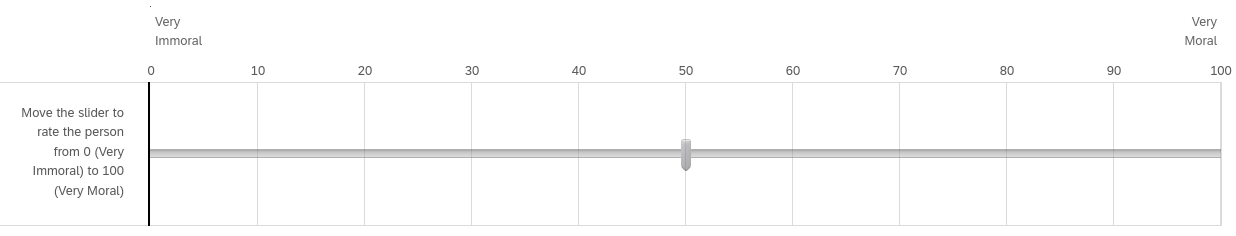
\includegraphics{../resources/images/mm1.png}
\caption{Screenshot of MM-1 as presented to participants}
\end{figure}

\newpage

\hypertarget{supplemantary-analyses}{%
\section{Supplemantary Analyses}\label{supplemantary-analyses}}

\hypertarget{supplementary-analyses}{%
\section{Supplementary Analyses}\label{supplementary-analyses}}

\hypertarget{pilot-study-1}{%
\section{Pilot Study 1}\label{pilot-study-1}}

\hypertarget{pilot-1-differences-between-moral-descriptions}{%
\subsection{Pilot: 1: Differences Between Moral Descriptions}\label{pilot-1-differences-between-moral-descriptions}}

We developed a combined moral perception measure by calculating the mean of the combined mean-centered scores for MPS-4 and MM-1, and mean-centering this result. Below we report the analyses for this combined measure.

The standardized means and standard deviations for the combined measure for each scenario are as follows:
\emph{Sam} (diagnostic),
\emph{M} = -0.30, \emph{SD} = 1.16;
\emph{Francis} (diagnostic),
\emph{M} = -0.22, \emph{SD} = 1.06;
\emph{Alex} (diagnostic),
\emph{M} = -0.25, \emph{SD} = 1.10;
\emph{Robin} (diagnostic),
\emph{M} = -0.31, \emph{SD} = 1.19;
\emph{Jackie} (non-diagnostic),
\emph{M} = 0.36, \emph{SD} = 0.55;
\emph{Charlie} (non-diagnostic),
\emph{M} = 0.35, \emph{SD} = 0.55. For the moral descriptions, we observed significant variation depending on the description, \emph{F}(3,602) = 2.67, \emph{p} = .050, partial \(\eta\)\textsuperscript{2} = 0.001. When correcting for multiple comparisons, pairwise comparisons did not reveal significant differences between descriptions. We note that without correction, \emph{Francis} appeared to be rated as more moral than both \emph{Robin} (\emph{p} = .022), and \emph{Sam} (\emph{p} = .021). For the neutral descriptions there was no significant difference in ratings depending on description, \emph{t}(211) = -0.46, \emph{p} = .645, \emph{d} = 0.03.

\hypertarget{pilot-1-testing-moral-vs-neutral}{%
\subsection{Pilot 1: Testing Moral vs Neutral}\label{pilot-1-testing-moral-vs-neutral}}

Overall, the model significantly predicted participants responses, and provided a better fit for the data than the baseline model \(\chi\)\textsuperscript{2}(2) = 1,035.36, \emph{p} \textless{} .001, and condition was a significant predictor in the model \(b\) = -0.31, \emph{t}(210.99) = -8.74, \emph{p} \textless{} .001.

\begin{figure}[!h]
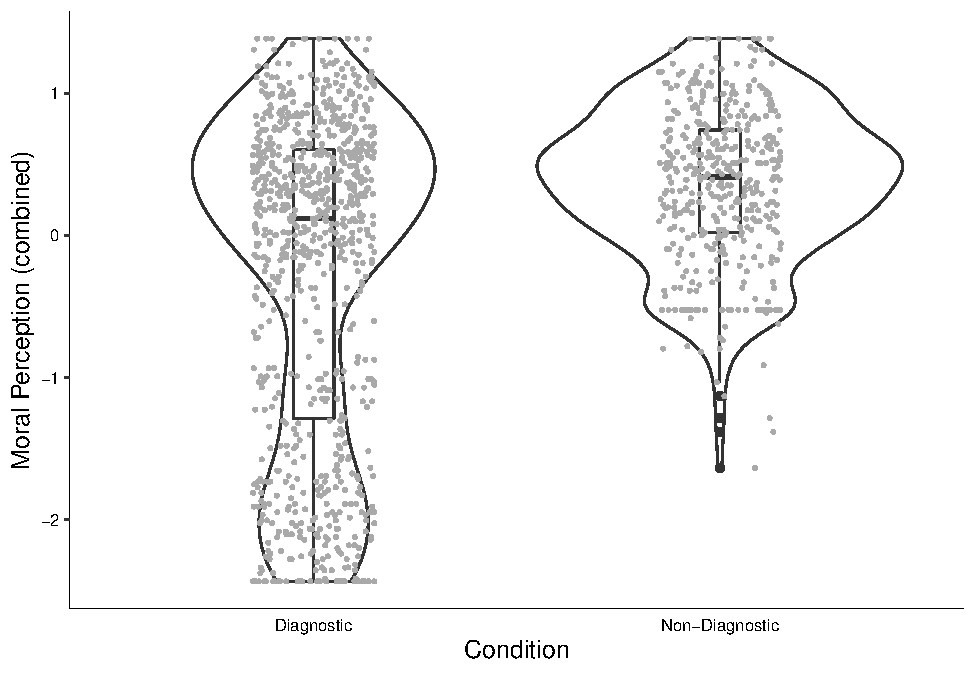
\includegraphics[width=\textwidth,]{Supplementary_files/figure-latex/pilot1cobminedconditionplot-1} \caption{Pilot Study 1: Differences in combined measure depending on condition}\label{fig:pilot1cobminedconditionplot}
\end{figure}

\newpage

\hypertarget{study-1}{%
\section{Study 1}\label{study-1}}

Again, we created a combined measure of moral perception from both DVs.

The means and standard deviations for the combined measure for each scenario are as follows:
\emph{Sam},
\emph{M} = 0.02, \emph{SD} = 0.89,
\emph{Francis},
\emph{M} = 0.48, \emph{SD} = 1.00,
\emph{Alex},
\emph{M} = -0.21, \emph{SD} = 0.92,
\emph{Robin},
\emph{M} = -0.32, \emph{SD} = 0.94. There was significant variation depending on the description, \emph{F}(3,2255) = 269.01, \emph{p} \textless{} .001, partial \(\eta\)\textsuperscript{2} = 0.10. \emph{Francis} appeared to be rated as the most favorable, followed by \emph{Sam}, then \emph{Alex} and finally \emph{Robin} as the least favorable (all \emph{p}s \textless{} .001).

We conducted a linear-mixed-effects model to test if condition influenced moral perception. Our outcome measure was the combined moral perception measure, our predictor variable was condition; we allowed intercepts and the effect of condition to vary across participants, and scenario was also included in the model.
Overall, the model significantly predicted participants responses, and provided a better fit for the data than the baseline model, \(\chi\)\textsuperscript{2}(8) = 762.31, \emph{p} \textless{} .001. Condition significantly influenced responses to the MPS-4, \emph{F}(1, 799.66) = 57.93, \emph{p} \textless{} .001; and was a significant predictor in the model when controlling for scenario, \(b\) = -0.08, \emph{t}(2,501.32) = -3.42, \emph{p} \textless{} .001, with the non-diagnostic descriptions being rated as more moral than the diagnostic (morally relevant) descriptions of immoral characters Figure~\ref{fig:S1combinedconditionplot}.

\begin{figure}[!h]
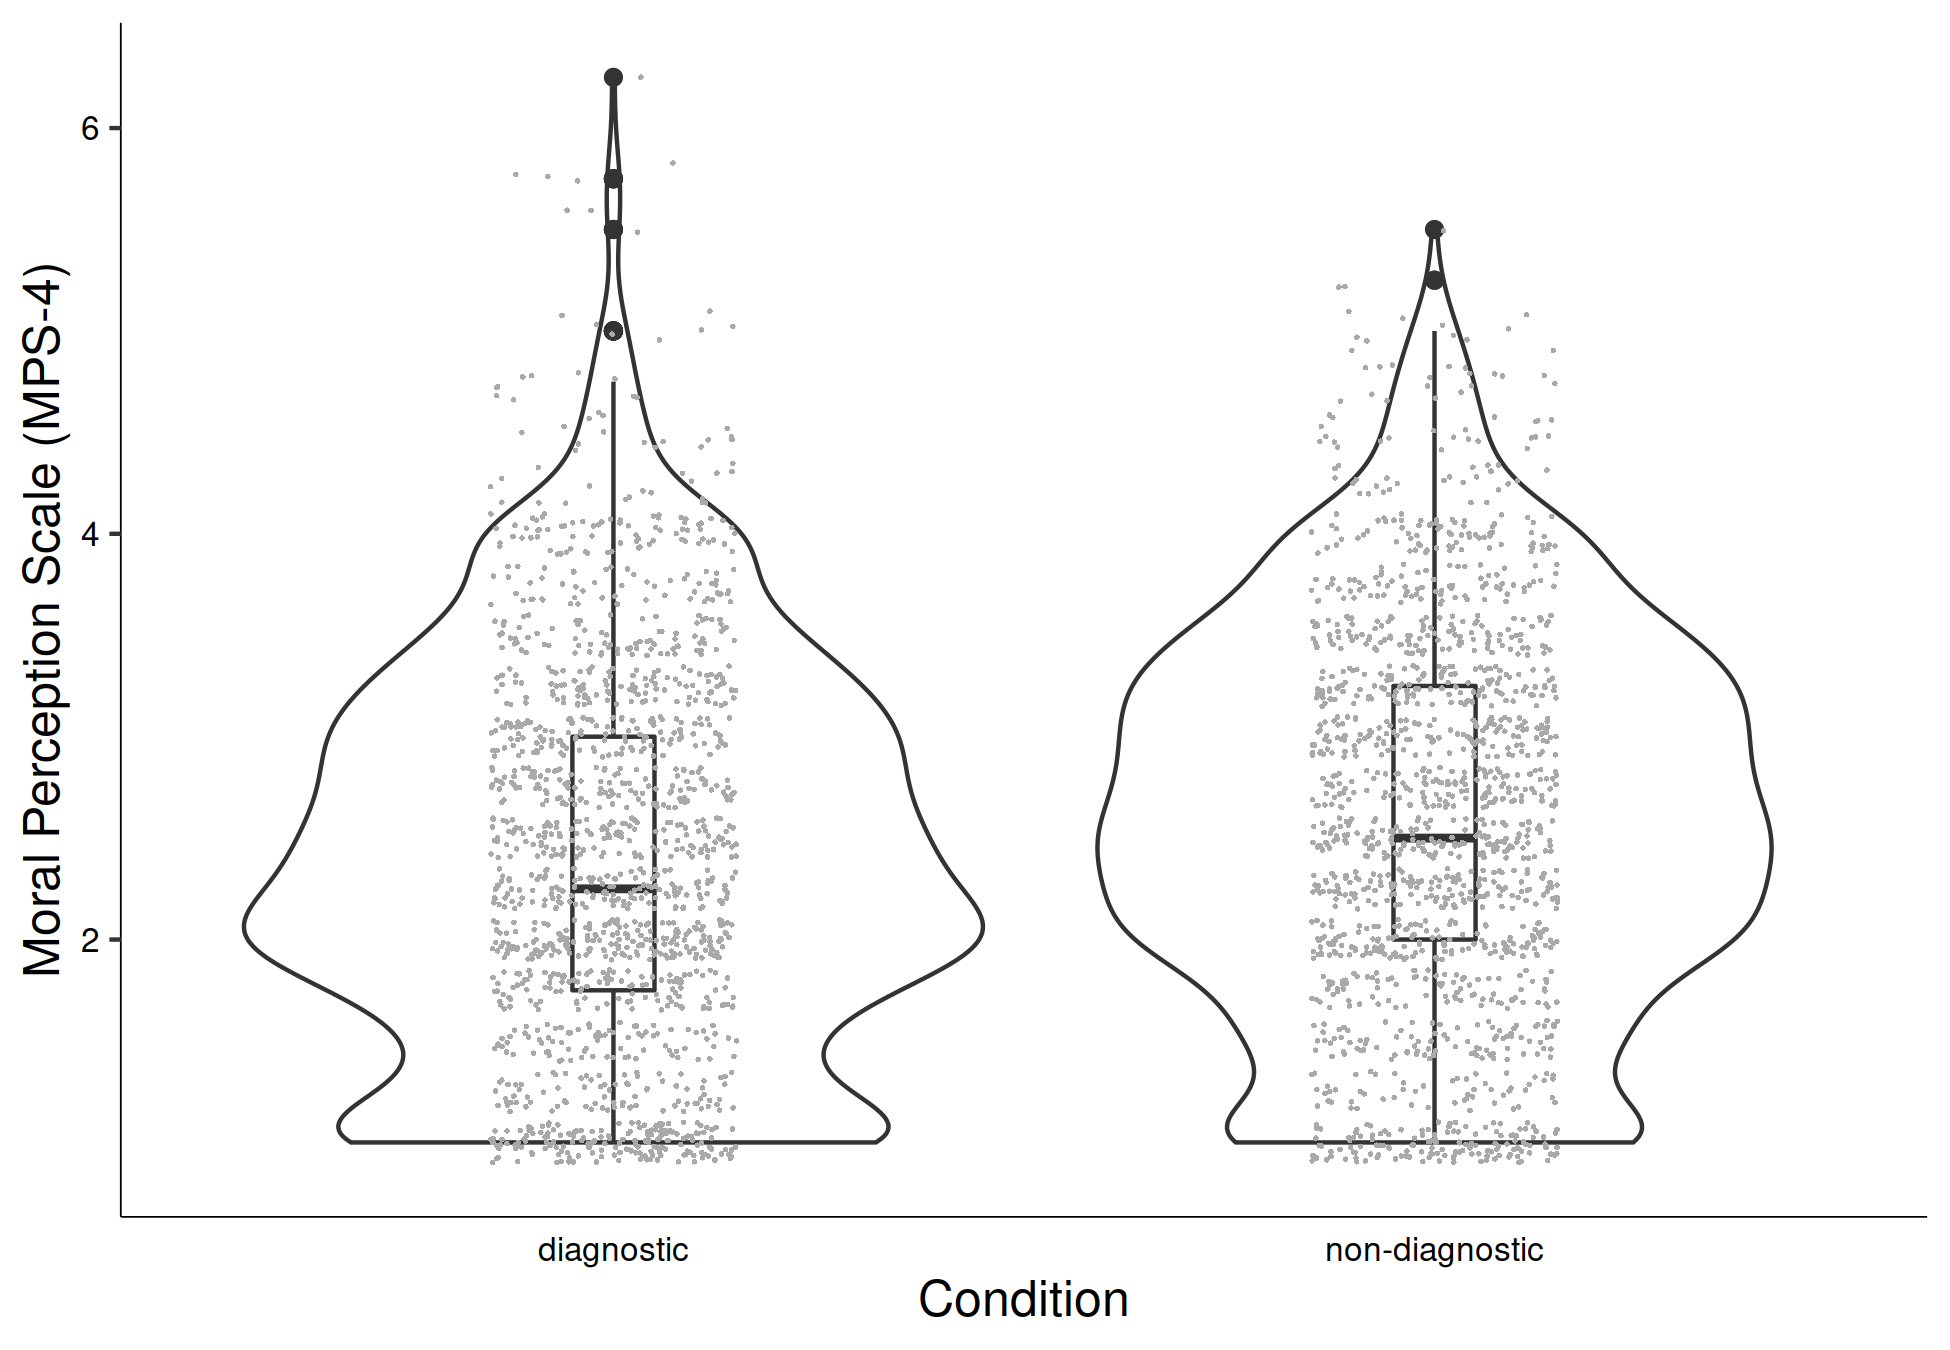
\includegraphics[width=\textwidth,]{Supplementary_files/figure-latex/S1combinedconditionplot-1} \caption{Study 1: Differences in combined measure depending on condition}\label{fig:S1combinedconditionplot}
\end{figure}

\hypertarget{study-1-differences-between-the-descriptions}{%
\subsection{Study 1: Differences between the Descriptions}\label{study-1-differences-between-the-descriptions}}

\begin{figure}[!p]
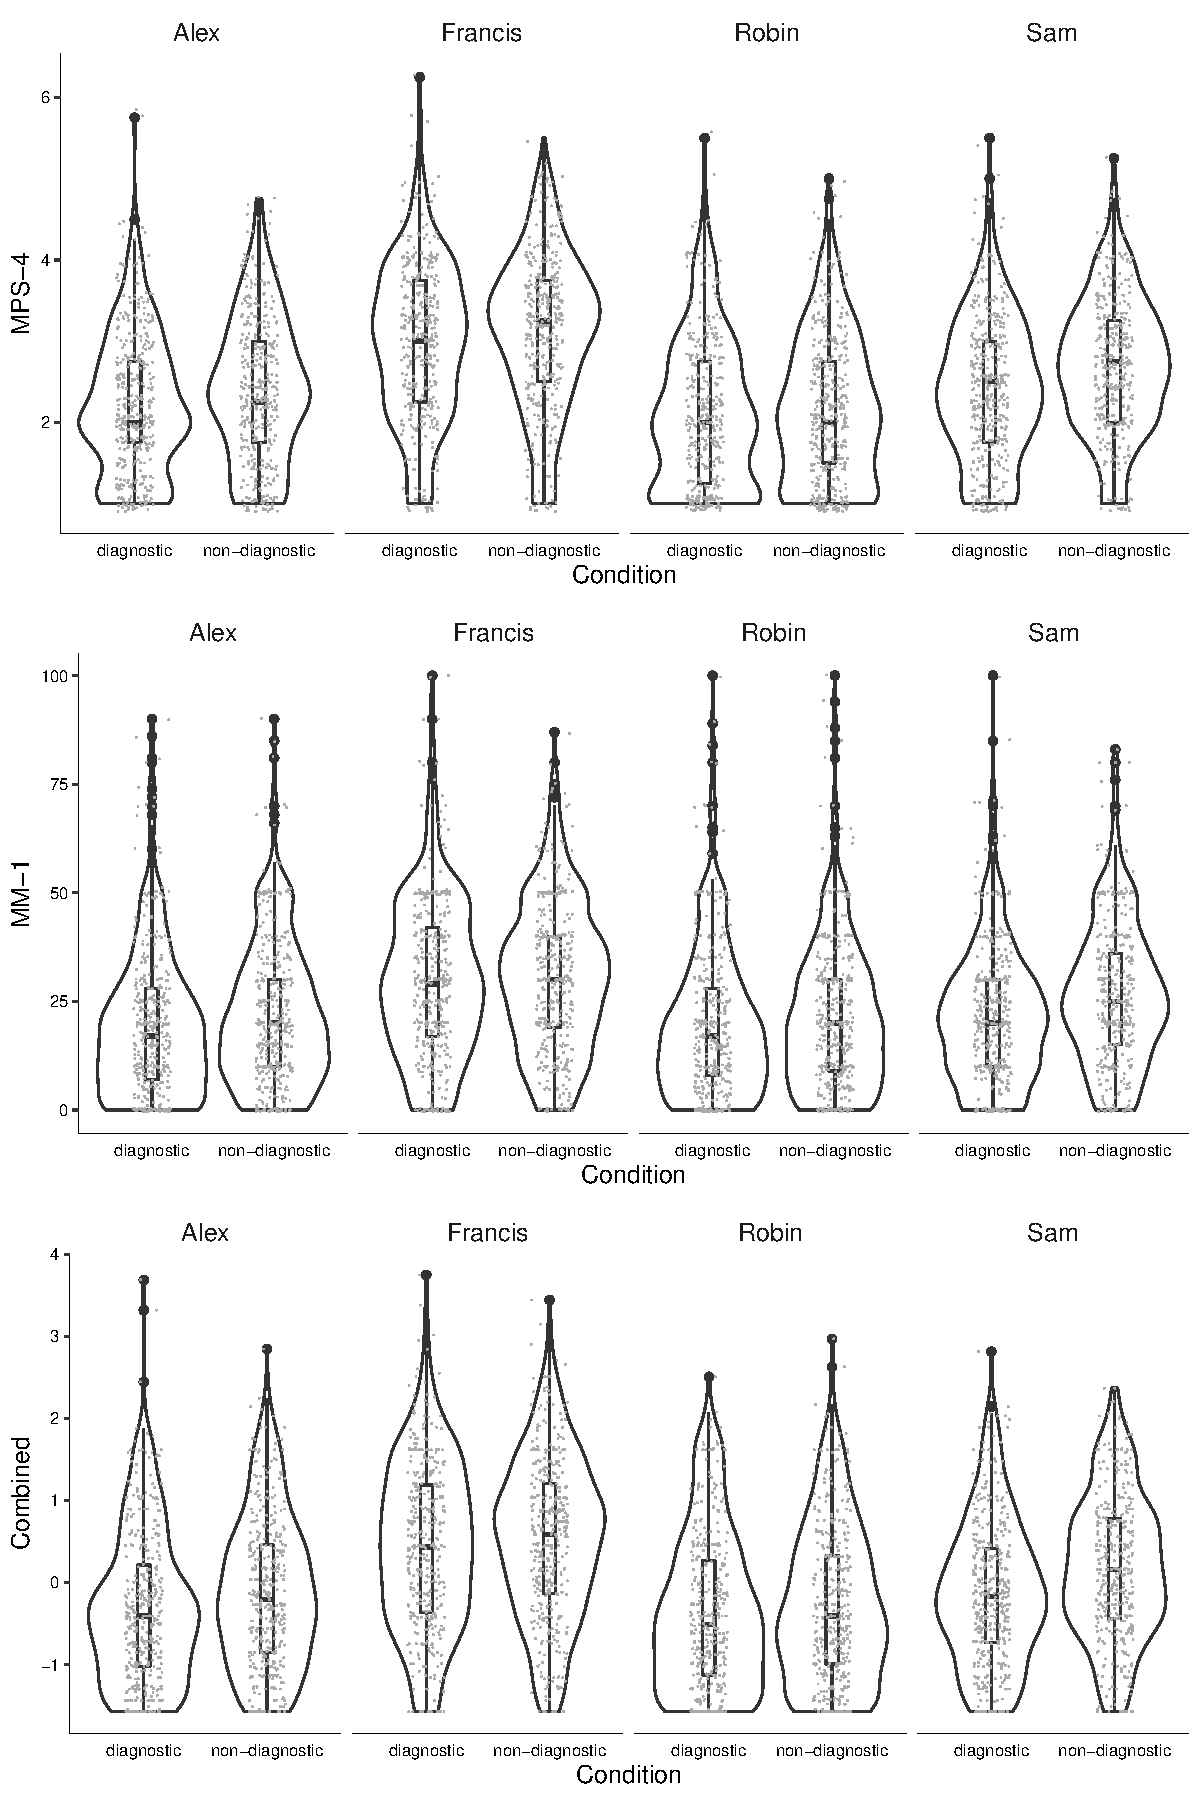
\includegraphics{Supplementary_files/figure-latex/S1allscenariosPlot-1} \caption{Study 1: Differences in moral perception for each description}\label{fig:S1allscenariosPlot}
\end{figure}

For \emph{Sam}, MPS-4 scores were significantly higher for the non-diagnostic condition (\emph{M} = 2.70, \emph{SD} = 0.82), than in the diagnostic condition (\emph{M} = 2.42, \emph{SD} = 0.87), \emph{t}(798.90) = -4.66, \emph{p} \textless{} .001, \emph{d} = 0.33; MM-1 ratings were higher in the non-diagnostic condition (\emph{M} = 26.55, \emph{SD} = 16.41), than in the diagnostic condition (\emph{M} = 21.50, \emph{SD} = 15.59), \emph{t}(787.84) = -4.45, \emph{p} \textless{} .001, \emph{d} = 0.32. For the combined measure ratings were also higher in the non-diagnostic condition (\emph{M} = 0.18, \emph{SD} = 0.88), than in the diagnostic condition (\emph{M} = -0.13, \emph{SD} = 0.88), \emph{t}(795.41) = -4.98, \emph{p} \textless{} .001, \emph{d} = 0.35.

For \emph{Robin}, MPS-4 scores were not significantly different for the non-diagnostic condition (\emph{M} = 2.16, \emph{SD} = 0.90), than in the diagnostic condition (\emph{M} = 2.09, \emph{SD} = 0.92), \emph{t}(793.94) = -1.09, \emph{p} = .275, \emph{d} = 0.08; MM-1 ratings were similar in the non-diagnostic condition (\emph{M} = 21.29, \emph{SD} = 16.94), and in the diagnostic condition (\emph{M} = 19.87, \emph{SD} = 17.17), \emph{t}(794.97) = -1.18, \emph{p} = .239, \emph{d} = 0.08. For the combined measure ratings were also similar in the non-diagnostic condition (\emph{M} = -0.28, \emph{SD} = 0.94), than in the diagnostic condition (\emph{M} = -0.36, \emph{SD} = 0.94), \emph{t}(796.03) = -1.24, \emph{p} = .217, \emph{d} = 0.09.

For \emph{Alex}, MPS-4 scores were significantly higher for the non-diagnostic condition (\emph{M} = 2.41, \emph{SD} = 0.88), than in the diagnostic condition (\emph{M} = 2.23, \emph{SD} = 0.86), \emph{t}(796.97) = -2.92, \emph{p} = .004, \emph{d} = 0.21; MM-1 ratings were higher in the non-diagnostic condition (\emph{M} = 21.93, \emph{SD} = 16.47), than in the diagnostic condition (\emph{M} = 19.20, \emph{SD} = 16.73), \emph{t}(798.89) = -2.33, \emph{p} = .020, \emph{d} = 0.16. For the combined measure ratings were also higher in the non-diagnostic condition (\emph{M} = -0.12, \emph{SD} = 0.92), than in the diagnostic condition (\emph{M} = -0.30, \emph{SD} = 0.92), \emph{t}(798.40) = -2.82, \emph{p} = .005, \emph{d} = 0.20.

For \emph{Francis}, MPS-4 scores were significantly higher for the non-diagnostic condition (\emph{M} = 3.12, \emph{SD} = 0.95), than in the diagnostic condition (\emph{M} = 2.98, \emph{SD} = 0.97), \emph{t}(796.12) = -1.99, \emph{p} = .047, \emph{d} = 0.14; MM-1 ratings were not significantly different in the non-diagnostic condition (\emph{M} = 30.38, \emph{SD} = 17.17), than in the diagnostic condition (\emph{M} = 29.84, \emph{SD} = 18.56), \emph{t}(788.61) = -0.43, \emph{p} = .668, \emph{d} = 0.03. For the combined measure ratings were also similar in the non-diagnostic condition (\emph{M} = 0.53, \emph{SD} = 0.98), and in the diagnostic condition (\emph{M} = 0.44, \emph{SD} = 1.02), \emph{t}(794.36) = -1.29, \emph{p} = .198, \emph{d} = 0.09.

\newpage

\hypertarget{pilot-study-2}{%
\section{Pilot Study 2}\label{pilot-study-2}}

\hypertarget{pilot-2-differences-between-moral-descriptions}{%
\subsection{Pilot: 2: Differences Between Moral Descriptions}\label{pilot-2-differences-between-moral-descriptions}}

As in previous studies, we developed a combined moral perception measure by calculating the mean of the combined mean-centered scores for MPS-4 and MM-1, and mean-centering this result. Below we report the analyses for this combined measure.

The standardized means and standard deviations for the combined measure for each scenario are as follows:
\emph{Sam} (moral),
\emph{M} = 0.21, \emph{SD} = 0.91;
\emph{Francis} (moral),
\emph{M} = 0.10, \emph{SD} = 0.96;
\emph{Alex} (moral),
\emph{M} = 0.18, \emph{SD} = 0.94;
\emph{Robin} (moral),
\emph{M} = 0.16, \emph{SD} = 0.93;
\emph{Jackie} (neutral),
\emph{M} = -0.24, \emph{SD} = 1.01;
\emph{Charlie} (neutral),
\emph{M} = -0.30, \emph{SD} = 1.07. For the moral descriptions, we observed significant variation depending on the description, \emph{F}(3,588) = 2.90, \emph{p} = .039, partial \(\eta\)\textsuperscript{2} = 0.002\emph{Sam} was viewed significantly more favorably than \emph{Francis} (\emph{p} = .045). For the neutral descriptions there was no significant difference in ratings depending on description, \emph{t}(214) = -1.46, \emph{p} = .147, \emph{d} = 0.10.

\newpage

\hypertarget{pilot-2-testing-moral-vs-neutral}{%
\subsection{Pilot 2: Testing Moral vs Neutral}\label{pilot-2-testing-moral-vs-neutral}}

Overall, the model significantly predicted participants responses, and provided a better fit for the data than the baseline model \(\chi\)\textsuperscript{2}(2) = 564.98, \emph{p} \textless{} .001, and condition was a significant predictor in the model \(b\) = 0.22, \emph{t}(214.32) = 6.60, \emph{p} \textless{} .001.

\begin{figure}[!h]
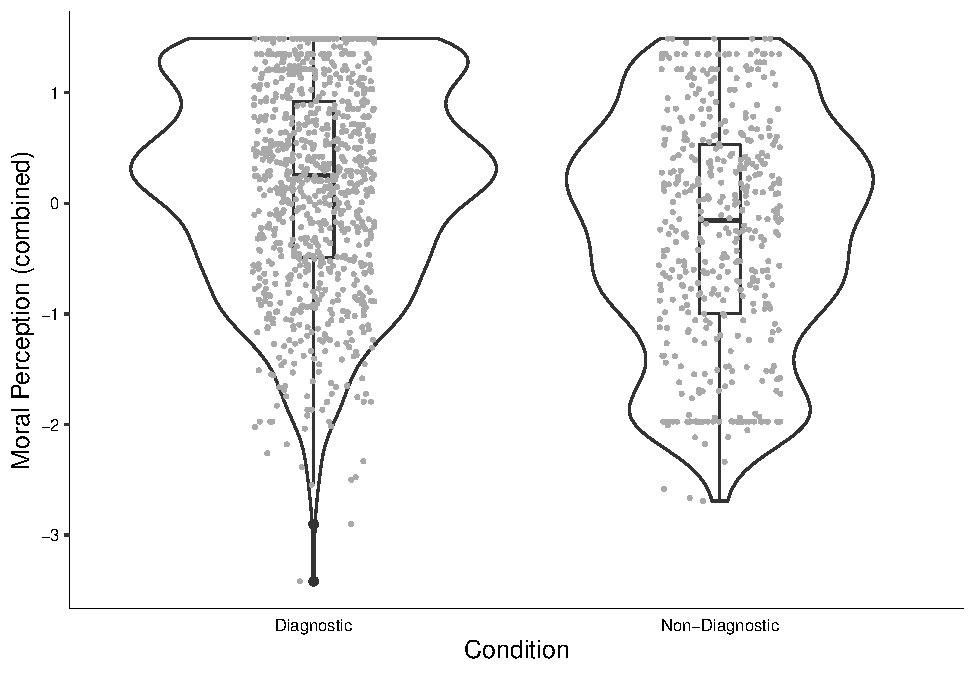
\includegraphics[width=\textwidth,]{Supplementary_files/figure-latex/pilot2cobminedconditionplot-1} \caption{Pilot Study 1: Differences in combined measure depending on condition}\label{fig:pilot2cobminedconditionplot}
\end{figure}

\newpage

\hypertarget{study-2}{%
\section{Study 2}\label{study-2}}

Below we report the results for the combined measure of moral perception from both DVs. We additionally report the effect of condition on responses to each description individually

The means and standard deviations for the combined measure for each scenario are as follows:
\emph{Sam},
\emph{M} = 0.07, \emph{SD} = 0.97,
\emph{Francis},
\emph{M} = -0.17, \emph{SD} = 1.06,
\emph{Alex},
\emph{M} = 0.09, \emph{SD} = 1.02,
\emph{Robin},
\emph{M} = 0.07, \emph{SD} = 0.96. There was significant variation depending on the description, \emph{F}(3,2335) = 48.01, \emph{p} \textless{} .001, partial \(\eta\)\textsuperscript{2} = 0.01. \emph{Francis} appeared to be rated as the less favorable than all other characters (all \emph{p}s \textless{} .001).

We conducted a linear-mixed-effects model to test if condition influenced moral perception. Our outcome measure was the combined moral perception measure, our predictor variable was condition; we allowed intercepts and the effect of condition to vary across participants, and scenario was also included in the model.
Overall, the model significantly predicted participants responses, and provided a better fit for the data than the baseline model, \(\chi\)\textsuperscript{2}(8) = 142.42, \emph{p} \textless{} .001. Condition did not influence moral perception, \emph{F}(1, 2,452.92) = 0.88, \emph{p} = .349; and was not a significant predictor in the model when controlling for scenario, \(b\) = -0.01, \emph{t}(2,613.53) = -0.42, \emph{p} = .673, see Figure~\ref{fig:S3combinedconditionplot}.

\begin{figure}[!h]
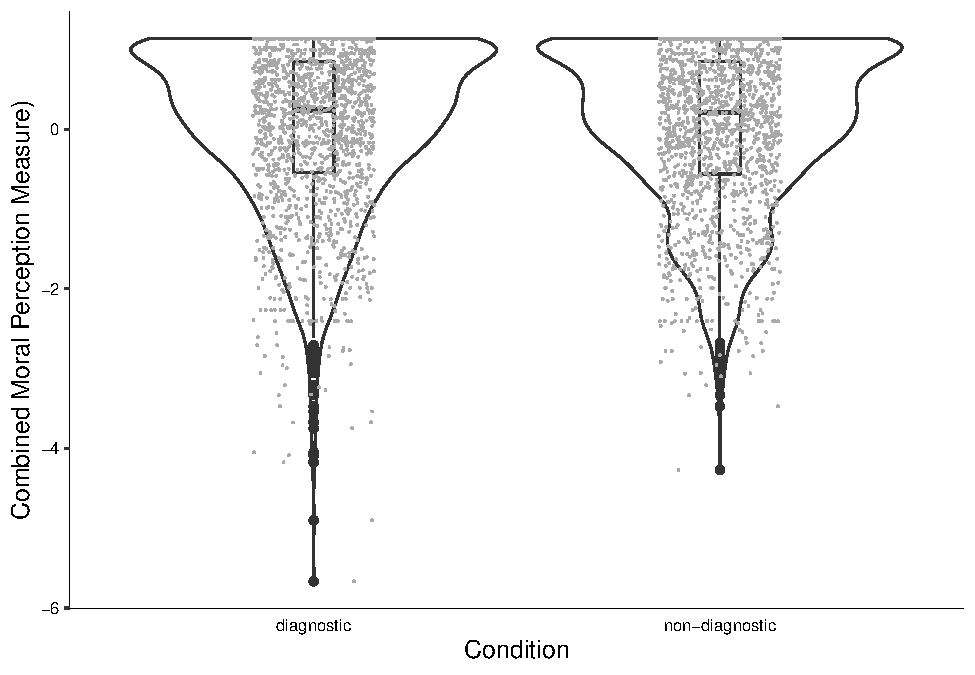
\includegraphics[width=\textwidth,]{Supplementary_files/figure-latex/S3combinedconditionplot-1} \caption{Study 2: Differences in combined measure depending on condition}\label{fig:S3combinedconditionplot}
\end{figure}

\newpage

\hypertarget{study-2-differences-between-the-descriptions}{%
\subsection{Study 2: Differences between the Descriptions}\label{study-2-differences-between-the-descriptions}}

\newpage

\begin{figure}[!p]
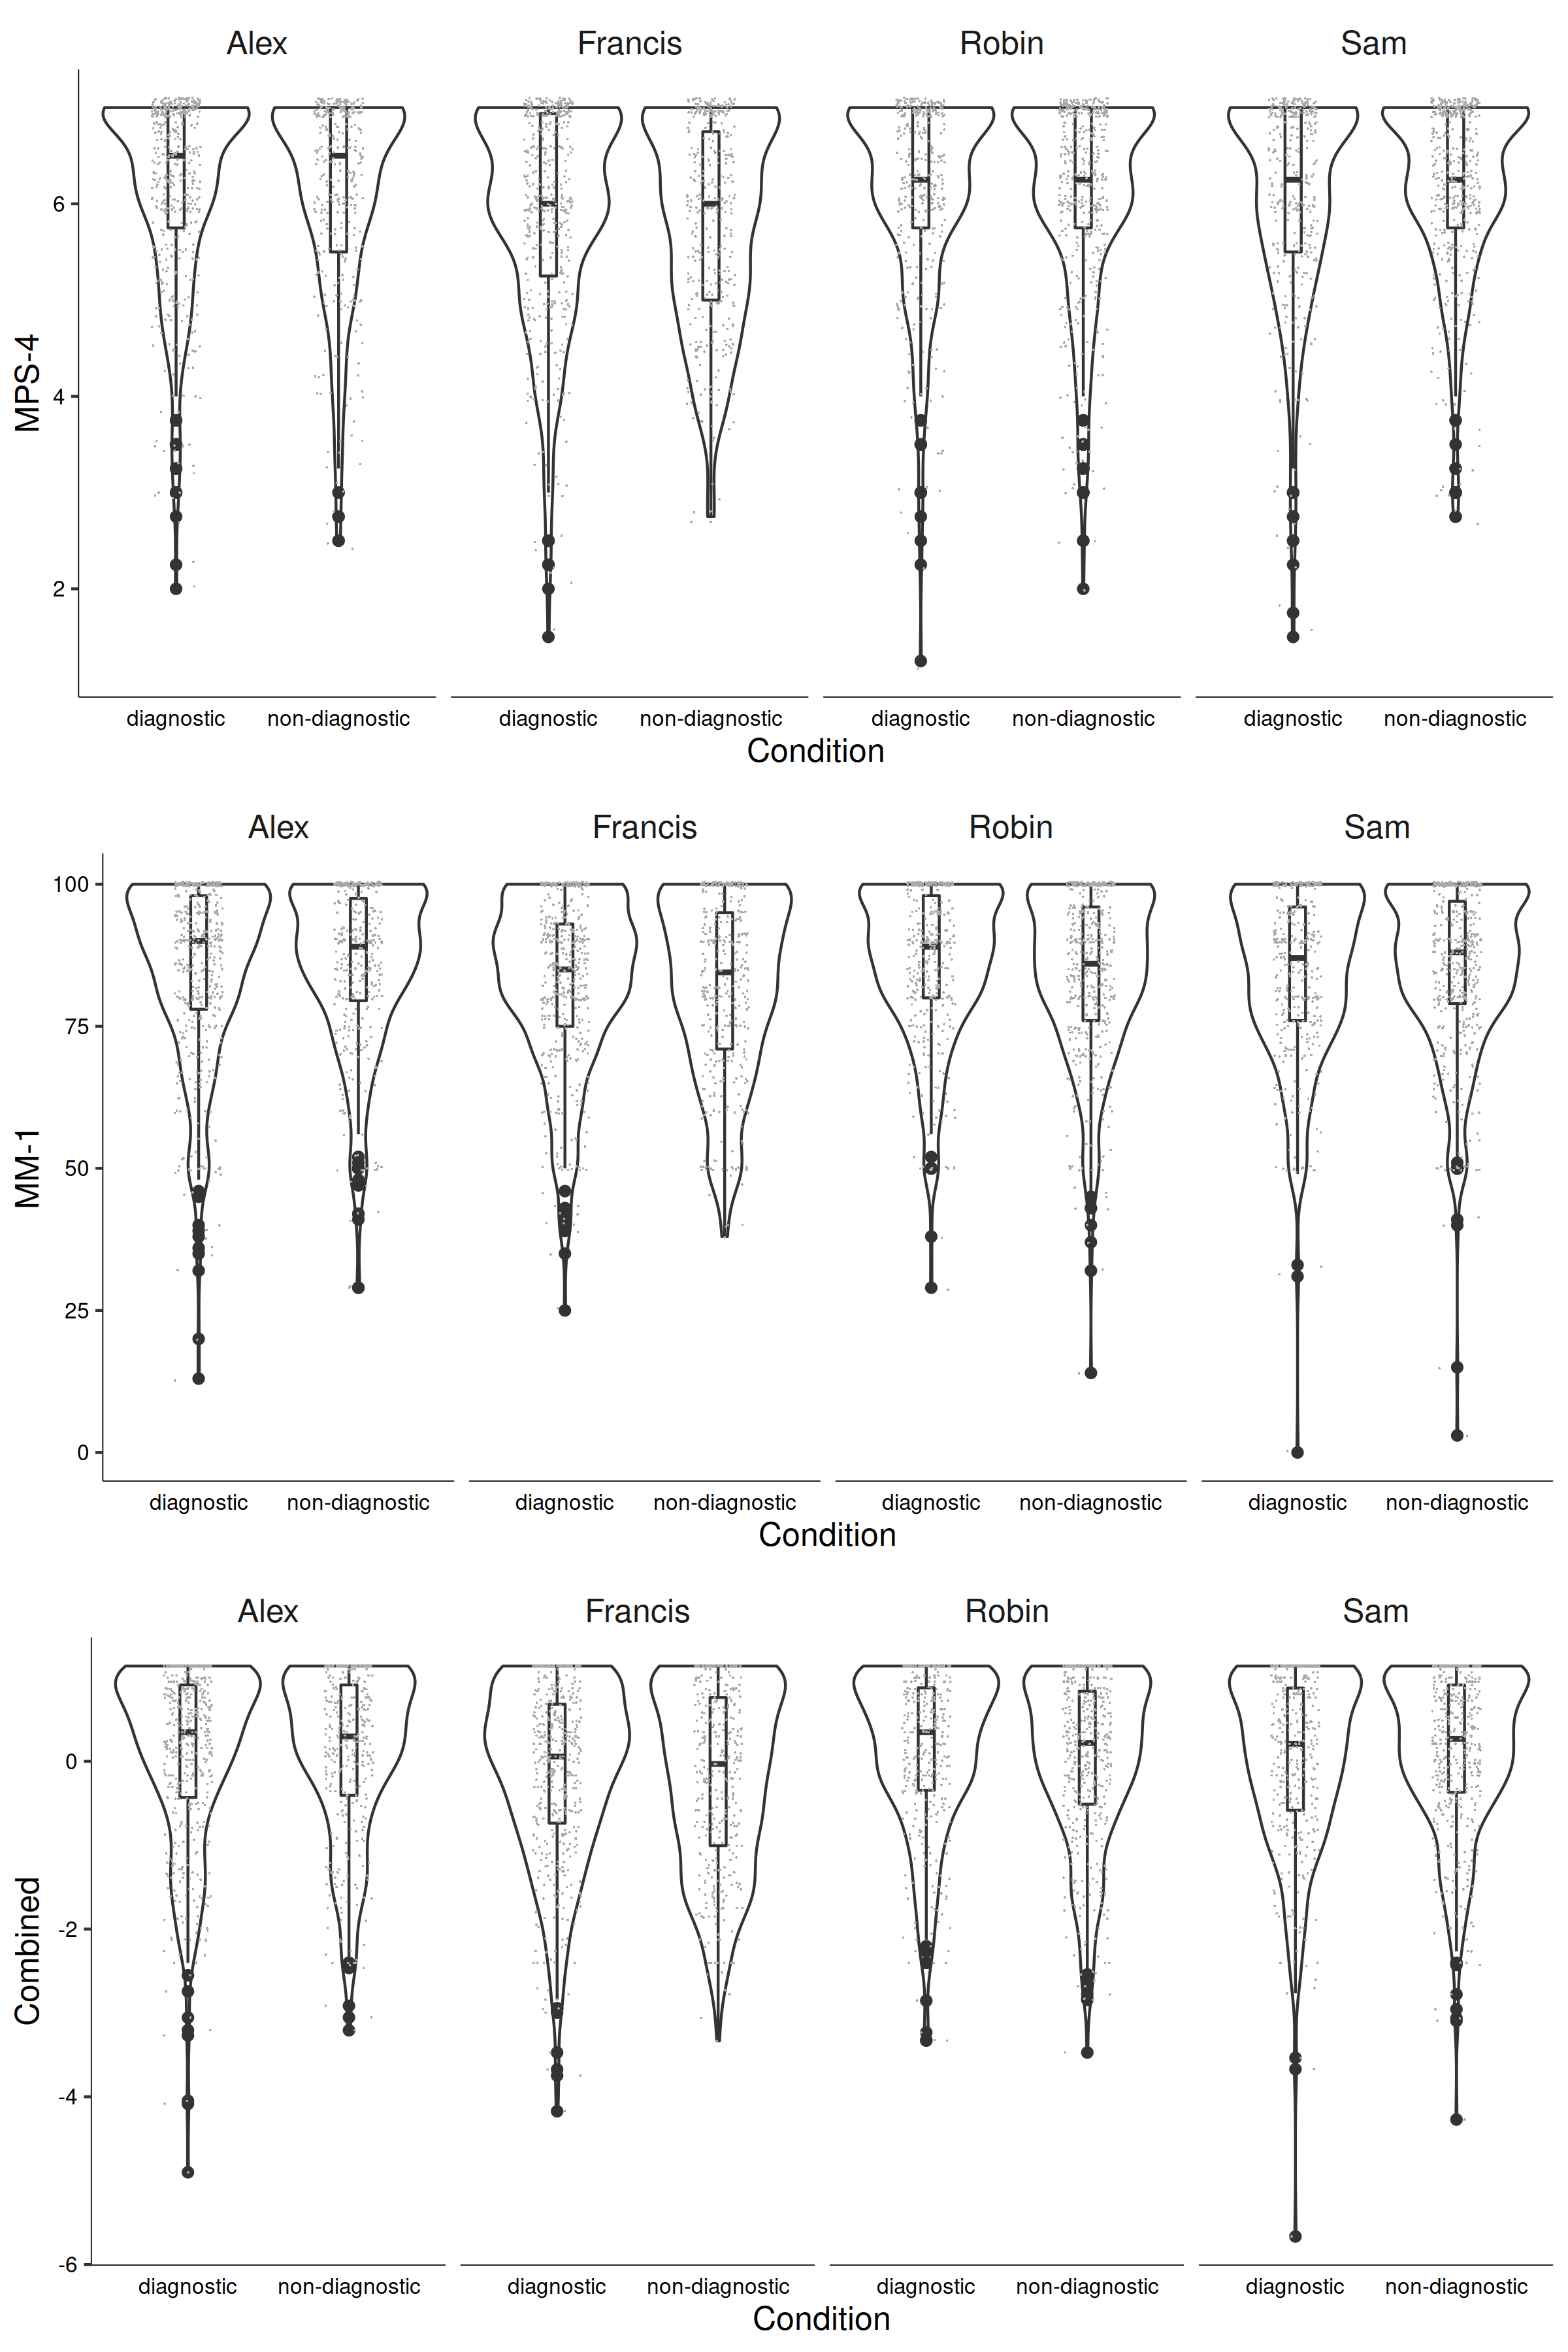
\includegraphics{Supplementary_files/figure-latex/S2allscenariosPlot-1} \caption{Study 2: Differences in moral perception for each description}\label{fig:S2allscenariosPlot}
\end{figure}

For \emph{Sam}, MPS-4 scores were not significantly different in the non-diagnostic condition (\emph{M} = 6.17, \emph{SD} = 0.89), than in the diagnostic condition (\emph{M} = 6.05, \emph{SD} = 1.06), \emph{t}(680.49) = -1.71, \emph{p} = .088, \emph{d} = 0.12; MM-1 ratings were similar in the non-diagnostic condition (\emph{M} = 84.90, \emph{SD} = 14.26), than in the diagnostic condition (\emph{M} = 84.20, \emph{SD} = 14.76), \emph{t}(744.17) = -0.69, \emph{p} = .490, \emph{d} = 0.05. For the combined measure ratings were also similar in the non-diagnostic condition (\emph{M} = 0.11, \emph{SD} = 0.93), than in the diagnostic condition (\emph{M} = 0.02, \emph{SD} = 1.03), \emph{t}(717.94) = -1.33, \emph{p} = .183, \emph{d} = 0.10.

For \emph{Robin}, MPS-4 scores were not significantly different for the non-diagnostic condition (\emph{M} = 6.08, \emph{SD} = 1.00), than in the diagnostic condition (\emph{M} = 6.13, \emph{SD} = 0.98), \emph{t}(784.04) = 0.73, \emph{p} = .463, \emph{d} = 0.05; MM-1 ratings were similar in the non-diagnostic condition (\emph{M} = 84.12, \emph{SD} = 14.37), and in the diagnostic condition (\emph{M} = 85.98, \emph{SD} = 13.32), \emph{t}(800.09) = 1.92, \emph{p} = .055, \emph{d} = 0.13. For the combined measure ratings were also similar in the non-diagnostic condition (\emph{M} = 0.03, \emph{SD} = 0.98), than in the diagnostic condition (\emph{M} = 0.13, \emph{SD} = 0.95), \emph{t}(788.76) = 1.46, \emph{p} = .145, \emph{d} = 0.10.

For \emph{Alex}, MPS-4 scores were not significantly different for the non-diagnostic condition (\emph{M} = 6.11, \emph{SD} = 1.00), than in the diagnostic condition (\emph{M} = 6.14, \emph{SD} = 0.99), \emph{t}(737.60) = 0.32, \emph{p} = .746, \emph{d} = 0.02; MM-1 ratings were similar in the non-diagnostic condition (\emph{M} = 85.28, \emph{SD} = 14.31), than in the diagnostic condition (\emph{M} = 84.83, \emph{SD} = 15.51), \emph{t}(776.47) = -0.43, \emph{p} = .668, \emph{d} = 0.03. For the combined measure ratings were also similar in the non-diagnostic condition (\emph{M} = 0.09, \emph{SD} = 0.98), than in the diagnostic condition (\emph{M} = 0.09, \emph{SD} = 1.04), \emph{t}(767.89) = -0.06, \emph{p} = .952, \emph{d} = 0.00.

For \emph{Francis}, MPS-4 scores were not significantly different for the non-diagnostic condition (\emph{M} = 5.82, \emph{SD} = 1.05), than in the diagnostic condition (\emph{M} = 5.90, \emph{SD} = 1.08), \emph{t}(794.94) = 1.06, \emph{p} = .290, \emph{d} = 0.07; MM-1 ratings were not significantly different in the non-diagnostic condition (\emph{M} = 81.74, \emph{SD} = 15.67), than in the diagnostic condition (\emph{M} = 82.31, \emph{SD} = 14.90), \emph{t}(771.23) = 0.54, \emph{p} = .591, \emph{d} = 0.04. For the combined measure ratings were also similar in the non-diagnostic condition (\emph{M} = -0.20, \emph{SD} = 1.08), and in the diagnostic condition (\emph{M} = -0.14, \emph{SD} = 1.04), \emph{t}(777.51) = 0.88, \emph{p} = .379, \emph{d} = 0.06.

\newpage

\newpage

\hypertarget{study-3}{%
\section{Study 3}\label{study-3}}

Below we report the results for the combined measure of moral perception from both DVs. We additionally report the effect of condition on responses to each description individually

The means and standard deviations for the combined measure for each scenario are as follows:
\emph{Sam},
\emph{M} = 0.45, \emph{SD} = 0.52,
\emph{Francis},
\emph{M} = -0.63, \emph{SD} = 1.19,
\emph{Alex},
\emph{M} = -0.66, \emph{SD} = 1.15,
\emph{Robin},
\emph{M} = 0.43, \emph{SD} = 0.52. There was significant variation depending on the description, \emph{F}(1,1027) = 473.77, \emph{p} \textless{} .001, partial \(\eta\)\textsuperscript{2} = 0.26. Both the \emph{good} characters (\emph{Robin} and \emph{Sam}) were rated significantly more favorably than both the \emph{bad} characters (\emph{Alex} and \emph{Francis}; all \emph{p}s \textless{} .001). There were no differences between \emph{Robin} and \emph{Sam} (\emph{good}: \emph{p} = .366) or between \emph{Alex} and \emph{Francis} (\emph{bad}; (\emph{p} = .648)).

We conducted a linear-mixed-effects model to test if our predictors influenced responses on the combined moral perception measure. Our outcome measure was the combined moral perception measure, our predictor variables were condition and valence; we allowed intercepts and the effects of condition and valence to vary across participants.
Overall, the model significantly predicted participants responses, and provided a better fit for the data than the baseline model,
\(\chi\)\textsuperscript{2}(5) = 3,889.20, \emph{p} \textless{} .001.
As expected, on its own, condition did not influence responses to the combined moral perception measure
, \emph{F}(1, 1746) = 0.02, \emph{p} = .876
; valence significantly predicted responses,
, \emph{F}(1, 1746) = 658.72, \emph{p} \textless{} .001
; and there was a significant condition \(\times\) valence interaction,
, \emph{F}(1, 1746) = 17.67, \emph{p} \textless{} .001.
and was not a significant predictor in the model when controlling for scenario, \(b\) = 0.00, \emph{t}(1,746.00) = -0.16, \emph{p} = .876, see Figure~\ref{fig:S3combinedplot}.

\begin{figure}[!h]
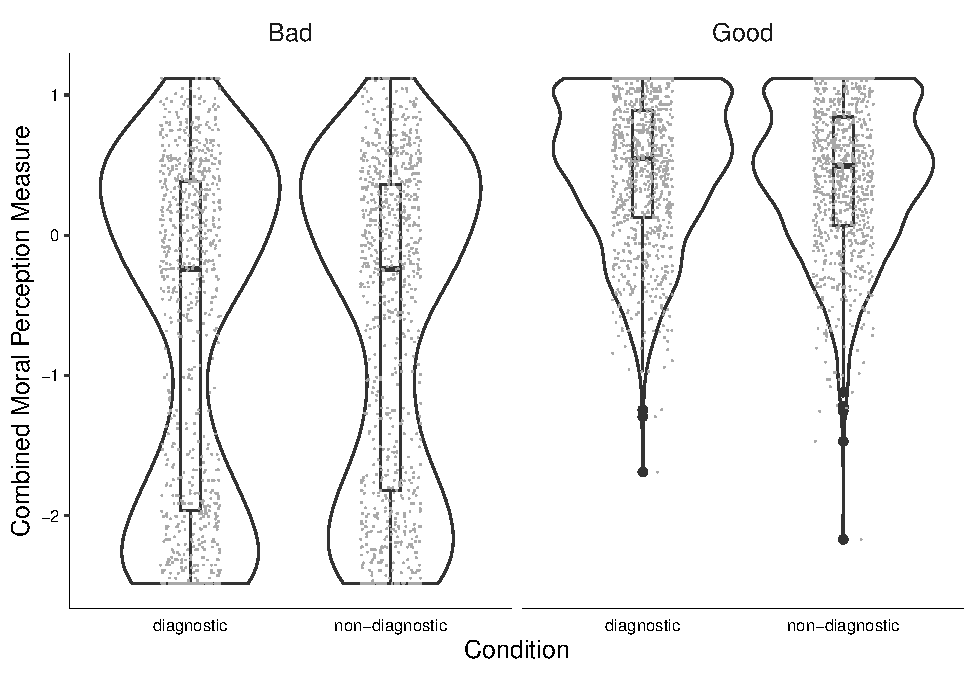
\includegraphics[width=\textwidth,]{Supplementary_files/figure-latex/S3combinedplot-1} \caption{Study 3: Differences in the combined measure depending on condition}\label{fig:S3combinedplot}
\end{figure}

\newpage

\hypertarget{study-3-differences-between-the-descriptions}{%
\subsection{Study 3: Differences between the descriptions}\label{study-3-differences-between-the-descriptions}}

\newpage

\begin{figure}[!p]
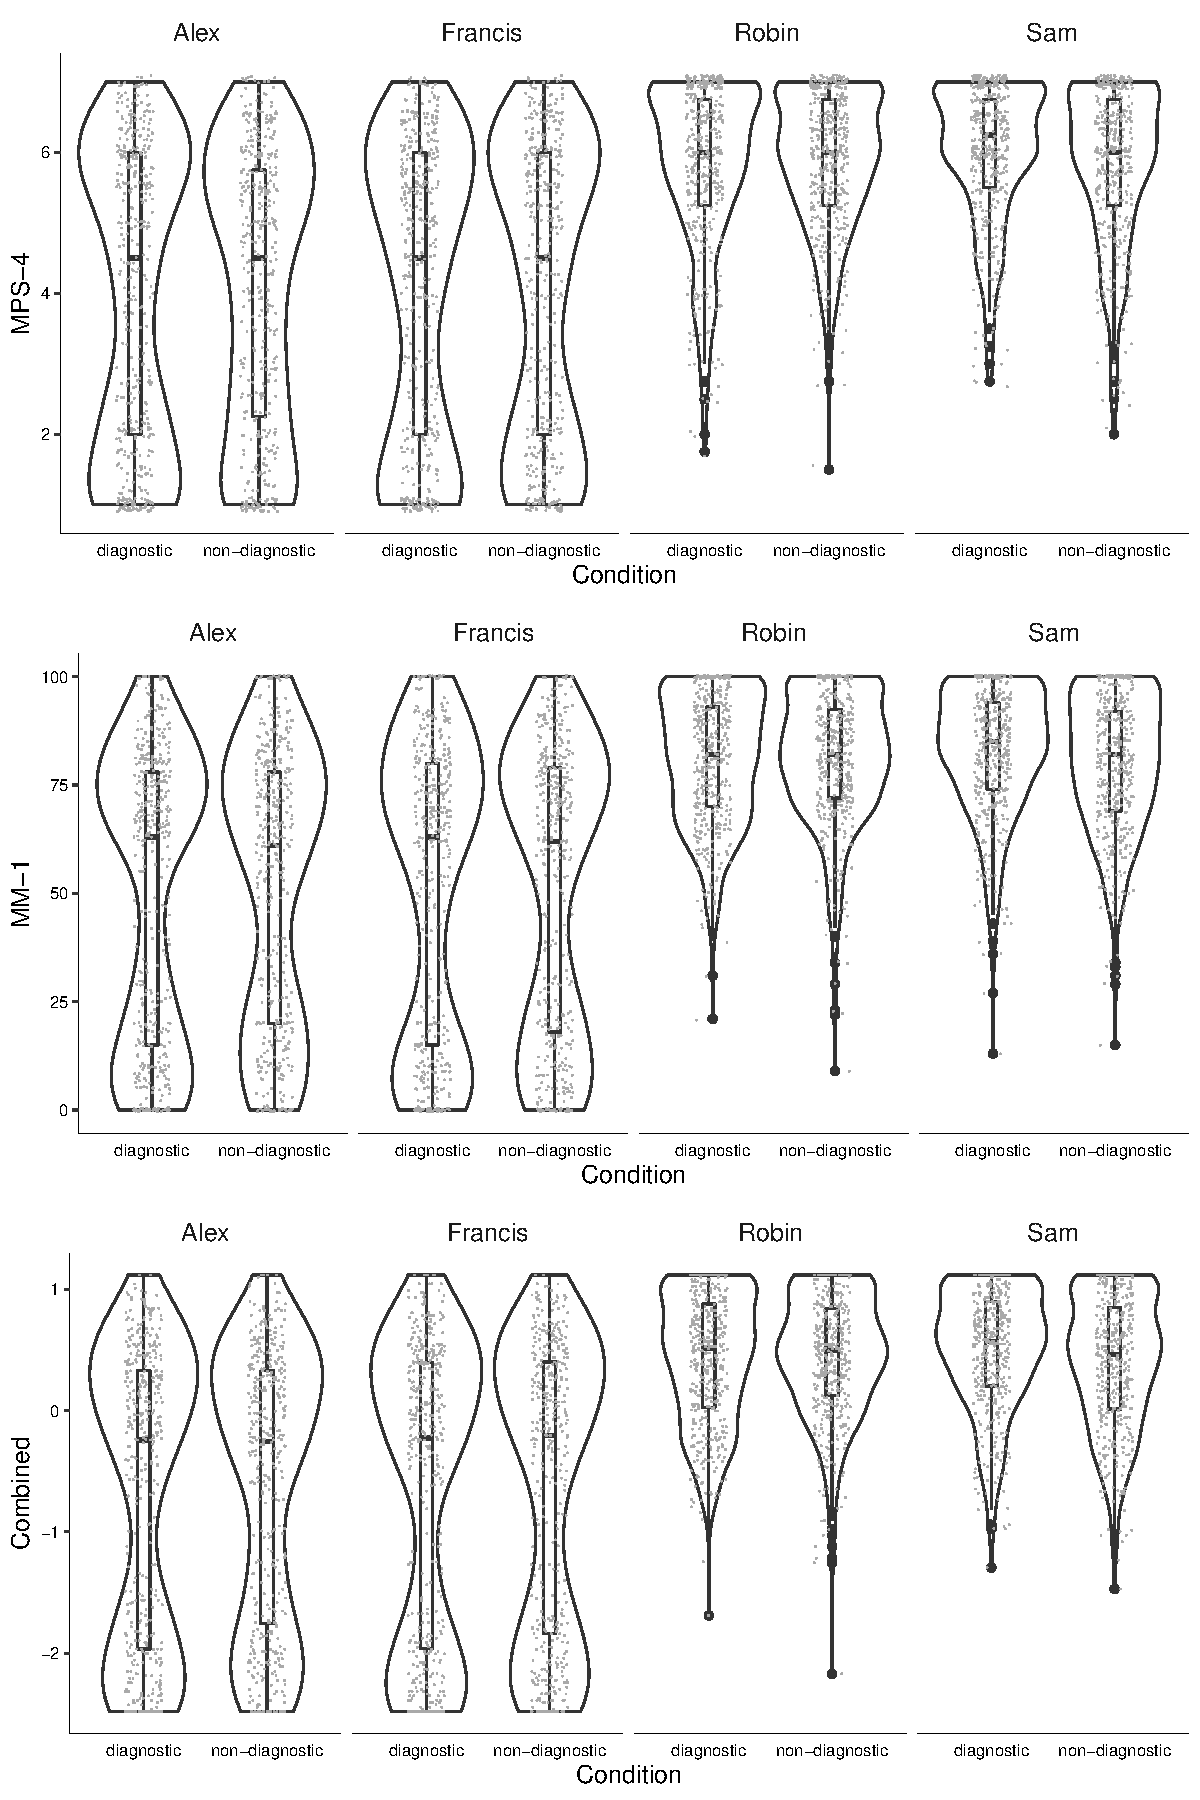
\includegraphics{Supplementary_files/figure-latex/S3allscenariosPlot-1} \caption{Study 3: Differences in moral perception for each description}\label{fig:S3allscenariosPlot}
\end{figure}

For \emph{Sam}, MPS-4 scores were significantly lower in the non-diagnostic condition (\emph{M} = 5.81, \emph{SD} = 1.09), than in the diagnostic condition (\emph{M} = 5.98, \emph{SD} = 0.97), \emph{t}(859.15) = 2.46, \emph{p} = .014, \emph{d} = 0.17; Similarly, MM-1 ratings were significantly lower in the non-diagnostic condition (\emph{M} = 79.64, \emph{SD} = 15.68), than in the diagnostic condition (\emph{M} = 82.37, \emph{SD} = 14.67), \emph{t}(867.08) = 2.66, \emph{p} = .008, \emph{d} = 0.18. For the combined measure ratings were also lower in the non-diagnostic condition (\emph{M} = 0.39, \emph{SD} = 0.54), than in the diagnostic condition (\emph{M} = 0.50, \emph{SD} = 0.50), \emph{t}(863.14) = 2.85, \emph{p} = .004, \emph{d} = 0.19.

For \emph{Robin}, MPS-4 scores were not significantly different for the non-diagnostic condition (\emph{M} = 5.88, \emph{SD} = 0.96), than in the diagnostic condition (\emph{M} = 5.83, \emph{SD} = 1.14), \emph{t}(844.53) = -0.77, \emph{p} = .440, \emph{d} = 0.05; MM-1 ratings were similar in the non-diagnostic condition (\emph{M} = 80.92, \emph{SD} = 15.27), and in the diagnostic condition (\emph{M} = 80.70, \emph{SD} = 15.07), \emph{t}(871.98) = -0.22, \emph{p} = .828, \emph{d} = 0.01. For the combined measure ratings were also similar in the non-diagnostic condition (\emph{M} = 0.44, \emph{SD} = 0.51), than in the diagnostic condition (\emph{M} = 0.42, \emph{SD} = 0.54), \emph{t}(867.63) = -0.57, \emph{p} = .569, \emph{d} = 0.04.

For \emph{Alex}, MPS-4 scores were not significantly different for the non-diagnostic condition (\emph{M} = 4.08, \emph{SD} = 1.96), than in the diagnostic condition (\emph{M} = 3.97, \emph{SD} = 2.11), \emph{t}(865.81) = -0.80, \emph{p} = .421, \emph{d} = 0.05; MM-1 ratings were similar in the non-diagnostic condition (\emph{M} = 52.19, \emph{SD} = 31.29), than in the diagnostic condition (\emph{M} = 49.58, \emph{SD} = 32.95), \emph{t}(868.76) = -1.20, \emph{p} = .230, \emph{d} = 0.08. For the combined measure ratings were also similar in the non-diagnostic condition (\emph{M} = -0.62, \emph{SD} = 1.11), than in the diagnostic condition (\emph{M} = -0.70, \emph{SD} = 1.19), \emph{t}(867.67) = -1.04, \emph{p} = .301, \emph{d} = 0.07.

For \emph{Francis}, MPS-4 scores were not significantly different for the non-diagnostic condition (\emph{M} = 4.08, \emph{SD} = 2.07), than in the diagnostic condition (\emph{M} = 4.07, \emph{SD} = 2.07), \emph{t}(871.94) = -0.09, \emph{p} = .928, \emph{d} = 0.01; MM-1 ratings were not significantly different in the non-diagnostic condition (\emph{M} = 51.56, \emph{SD} = 32.68), than in the diagnostic condition (\emph{M} = 51.42, \emph{SD} = 33.70), \emph{t}(871.59) = -0.06, \emph{p} = .952, \emph{d} = 0.00. For the combined measure ratings were also similar in the non-diagnostic condition (\emph{M} = -0.63, \emph{SD} = 1.18), and in the diagnostic condition (\emph{M} = -0.64, \emph{SD} = 1.20), \emph{t}(871.88) = -0.08, \emph{p} = .939, \emph{d} = 0.01.

\newpage

\hypertarget{study-4}{%
\section{Study 4}\label{study-4}}

Below we report the results for the combined measure of moral perception from both DVs. We additionally report the effect of condition on responses to each description individually

The means and standard deviations for the combined measure for each scenario are as follows:
\emph{Sam},
\emph{M} = 0.03, \emph{SD} = 1.02,
\emph{Francis},
\emph{M} = -0.03, \emph{SD} = 0.98,
\emph{Alex},
\emph{M} = 0.02, \emph{SD} = 1.04,
\emph{Robin},
\emph{M} = 0.04, \emph{SD} = 1.01. There was significant variation depending on the description, \emph{F}(3,2493) = 4.32, \emph{p} = .005, partial \(\eta\)\textsuperscript{2} = 0.00. \emph{Francis} appeared to be rated as the less favorable than all other characters (all \emph{p}s \textless{} .001).

We conducted a linear-mixed-effects model to test if condition influenced moral perception. Our outcome measure was the combined moral perception measure, our predictor variable was condition; we allowed intercepts and the effect of condition to vary across participants, and scenario was also included in the model.
Overall, the model significantly predicted participants responses, and provided a better fit for the data than the baseline model, \(\chi\)\textsuperscript{2}(8) = 42.42, \emph{p} \textless{} .001. Condition did not influence moral perception, \emph{F}(1, 865.01) = 5.31, \emph{p} = .021; and was not a significant predictor in the model when controlling for scenario, \(b\) = -0.01, \emph{t}(2,541.03) = -0.82, \emph{p} = .410, see Figure~\ref{fig:S3combinedconditionplot}.

\begin{figure}[!h]
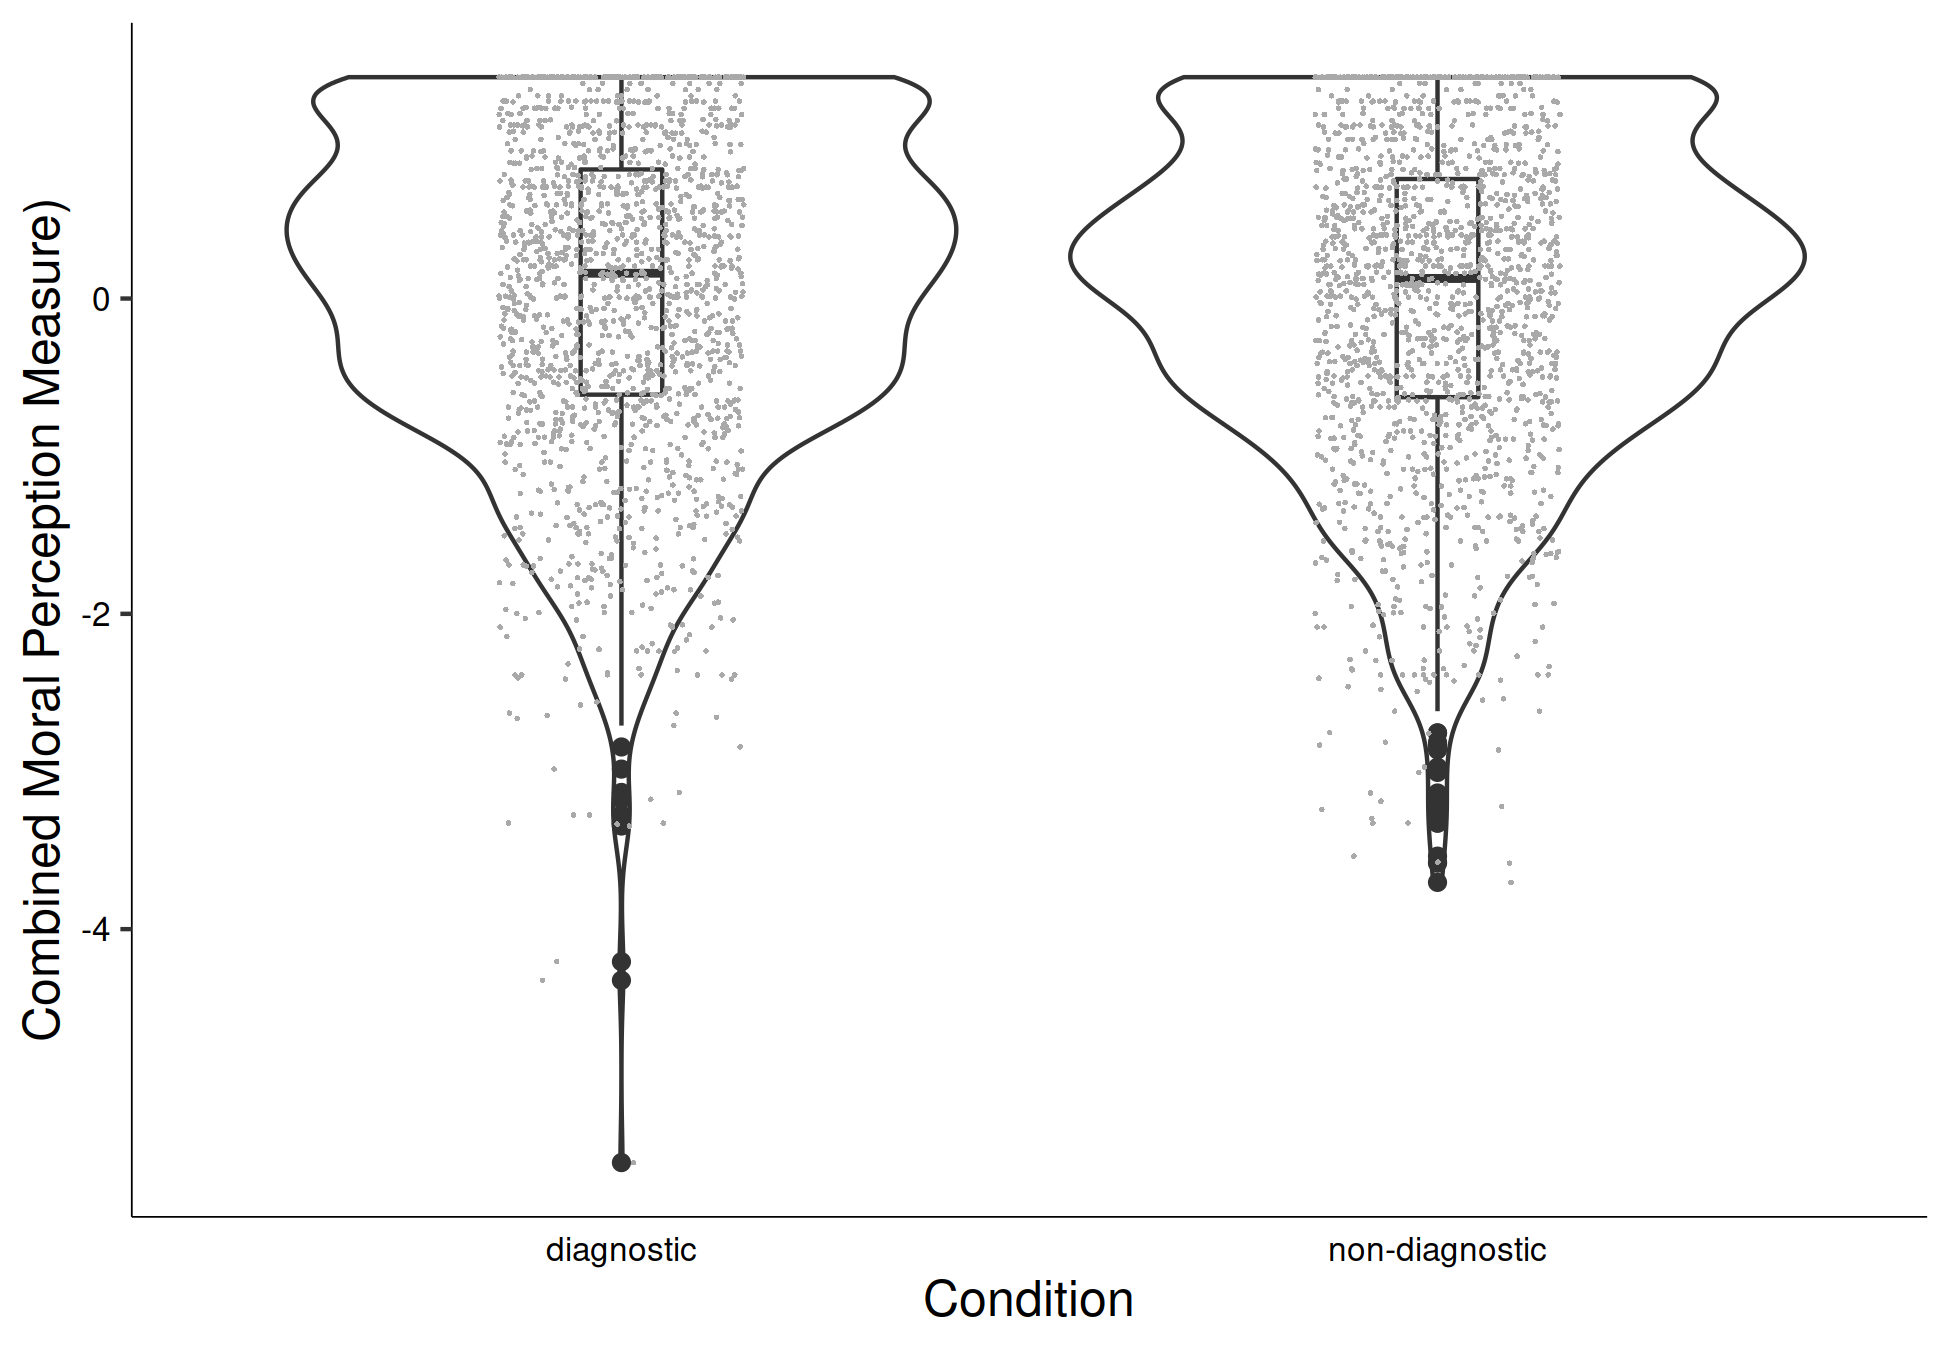
\includegraphics[width=\textwidth,]{Supplementary_files/figure-latex/S4combinedconditionplot-1} \caption{Study 4: Differences in combined measure depending on condition}\label{fig:S4combinedconditionplot}
\end{figure}

\newpage

\hypertarget{study-4-differences-between-the-descriptions}{%
\subsection{Study 4: Differences between the Descriptions}\label{study-4-differences-between-the-descriptions}}

\newpage

\begin{figure}[!p]
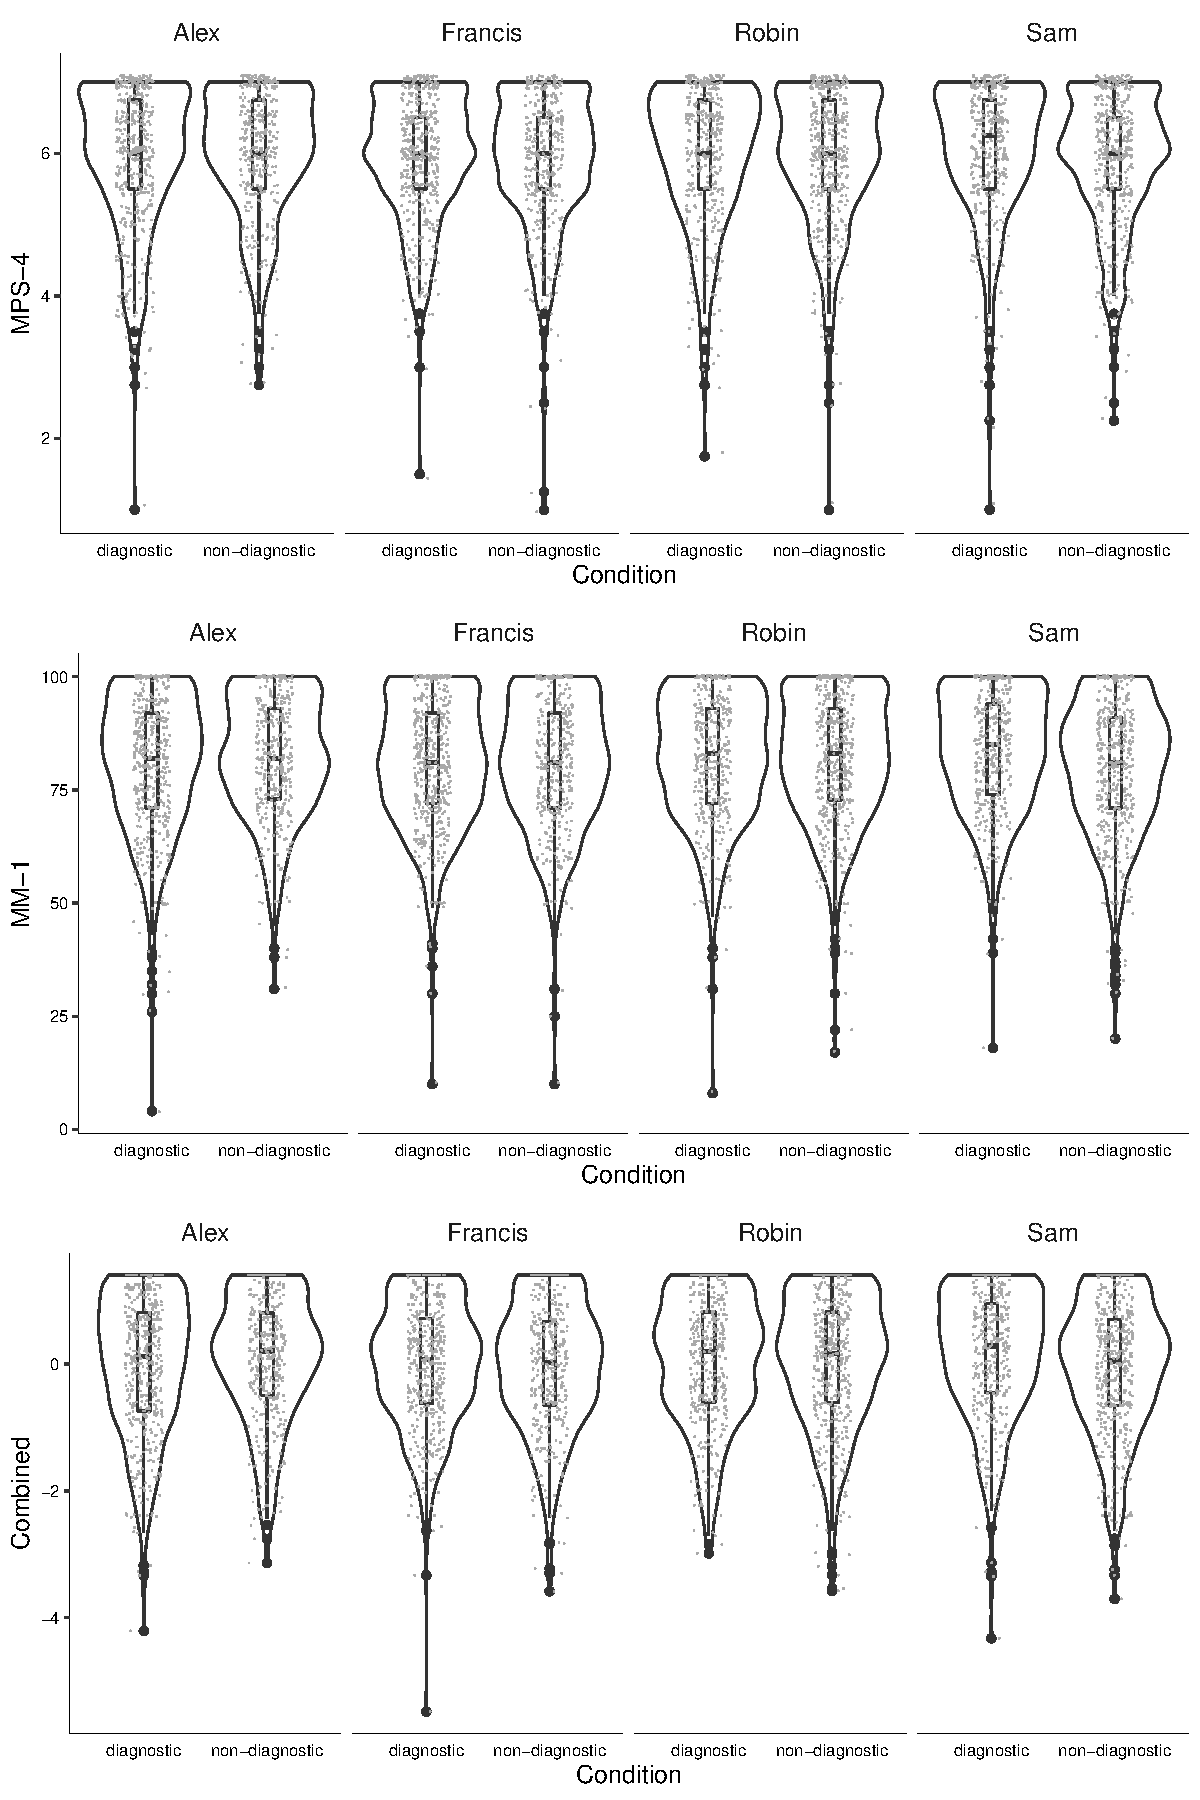
\includegraphics{Supplementary_files/figure-latex/S4allscenariosPlot-1} \caption{Study 4: Differences in moral perception for each description}\label{fig:S4allscenariosPlot}
\end{figure}

For \emph{Sam} (good), MPS-4 scores were significantly lower in the non-diagnostic condition (\emph{M} = 5.89, \emph{SD} = 0.91), than in the diagnostic condition (\emph{M} = 6.02, \emph{SD} = 0.95), \emph{t}(810.53) = 1.97, \emph{p} = .049, \emph{d} = 0.14; MM-1 ratings were similar in the non-diagnostic condition (\emph{M} = 79.75, \emph{SD} = 14.62), than in the diagnostic condition (\emph{M} = 83.25, \emph{SD} = 13.30), \emph{t}(845.88) = 3.66, \emph{p} \textless{} .001, \emph{d} = 0.25. For the combined measure ratings were also similar in the non-diagnostic condition (\emph{M} = -0.06, \emph{SD} = 1.03), than in the diagnostic condition (\emph{M} = 0.15, \emph{SD} = 1.01), \emph{t}(829.20) = 3.07, \emph{p} = .002, \emph{d} = 0.21.

For \emph{Robin} (good), MPS-4 scores were significantly lower for the non-diagnostic condition (\emph{M} = 5.95, \emph{SD} = 0.93), than in the diagnostic condition (\emph{M} = 5.94, \emph{SD} = 0.95), \emph{t}(811.83) = -0.20, \emph{p} = .841, \emph{d} = 0.01; MM-1 ratings were lower in the non-diagnostic condition (\emph{M} = 81.62, \emph{SD} = 14.28), than in the diagnostic condition (\emph{M} = 81.64, \emph{SD} = 14.02), \emph{t}(824.54) = 0.02, \emph{p} = .982, \emph{d} = 0.00. For the combined measure ratings were also lower in the non-diagnostic condition (\emph{M} = 0.04, \emph{SD} = 1.03), than in the diagnostic condition (\emph{M} = 0.04, \emph{SD} = 0.99), \emph{t}(828.47) = -0.10, \emph{p} = .919, \emph{d} = 0.01.

For \emph{Alex}, MPS-4 scores were not significantly different for the non-diagnostic condition (\emph{M} = 5.97, \emph{SD} = 0.91), than in the diagnostic condition (\emph{M} = 5.91, \emph{SD} = 0.99), \emph{t}(845.29) = -0.91, \emph{p} = .362, \emph{d} = 0.06; MM-1 ratings were similar in the non-diagnostic condition (\emph{M} = 81.93, \emph{SD} = 13.38), than in the diagnostic condition (\emph{M} = 80.51, \emph{SD} = 15.21), \emph{t}(850.53) = -1.46, \emph{p} = .145, \emph{d} = 0.10. For the combined measure ratings were also similar in the non-diagnostic condition (\emph{M} = 0.07, \emph{SD} = 0.98), than in the diagnostic condition (\emph{M} = -0.02, \emph{SD} = 1.09), \emph{t}(847.27) = -1.30, \emph{p} = .192, \emph{d} = 0.09.

For \emph{Francis}, MPS-4 scores were not significantly different for the non-diagnostic condition (\emph{M} = 5.87, \emph{SD} = 0.95), than in the diagnostic condition (\emph{M} = 5.91, \emph{SD} = 0.87), \emph{t}(787.36) = 0.77, \emph{p} = .443, \emph{d} = 0.05; MM-1 ratings were not significantly different in the non-diagnostic condition (\emph{M} = 80.54, \emph{SD} = 14.38), than in the diagnostic condition (\emph{M} = 80.75, \emph{SD} = 13.99), \emph{t}(809.63) = 0.21, \emph{p} = .832, \emph{d} = 0.01. For the combined measure ratings were also similar in the non-diagnostic condition (\emph{M} = -0.05, \emph{SD} = 0.99), and in the diagnostic condition (\emph{M} = -0.01, \emph{SD} = 0.98), \emph{t}(814.30) = 0.55, \emph{p} = .581, \emph{d} = 0.04.

\hypertarget{study-5}{%
\section{Study 5}\label{study-5}}

The means and standard deviations for the combined measure for each scenario are as follows:
\emph{Sam},
\emph{M} = 84.52, \emph{SD} = 15.49;
\emph{Francis},
\emph{M} = 44.51, \emph{SD} = 35.08;
\emph{Alex},
\emph{M} = 45.85, \emph{SD} = 34.36;
\emph{Robin},
\emph{M} = 85.15, \emph{SD} = 14.61. There was significant variation depending on the description, \emph{F}(3,1746) = 351.55, \emph{p} \textless{} .001, partial \(\eta\)\textsuperscript{2} = 0.38. Both the \emph{good} characters (\emph{Robin} and \emph{Sam}) were rated significantly more favorably than both the \emph{bad} characters (\emph{Alex} and \emph{Francis}; all \emph{p}s \textless{} .001). There were no differences between \emph{Robin} and \emph{Sam} (\emph{good}: \emph{p} = .963) or between \emph{Alex} and \emph{Francis} (\emph{bad}; (\emph{p} = .976)).

We conducted a 2 \(\times\) 2 between subjects ANOVA to test for an interaction between valence and condition.
As expected, on its own, condition did not influence responses to the MPS-4
, \emph{F}(1, 1746) = 0.09, \emph{p} = .767
; valence significantly predicted responses,
, \emph{F}(1, 1746) = 1,058.79, \emph{p} \textless{} .001
; and there was a significant condition \(\times\) valence interaction,
, \emph{F}(1, 1746) = 7.92, \emph{p} = .005.

For the \emph{bad} characters, there was no significant difference in responses to the combined measure between the diagnostic condition (\emph{M} = -0.81, \emph{SD} = 1.15) and the non-diagnostic condition (\emph{M} = -0.70, \emph{SD} = 1.07) depending on condition, \emph{t}(834.36) = -1.23, \emph{p} = .221, \emph{d} = 0.09.

For the \emph{good} characters, there was a significant difference in responses to the combined measure between the diagnostic condition (\emph{M} = 0.61, \emph{SD} = 0.41) and the non-diagnostic condition (\emph{M} = 0.49, \emph{SD} = 0.44) depending on condition, \emph{t}(886.55) = 3.16, \emph{p} = .002, \emph{d} = 0.28.

\hypertarget{study-5-differences-between-the-descriptions}{%
\subsection{Study 5: Differences between the Descriptions}\label{study-5-differences-between-the-descriptions}}

\begin{figure}[!p]
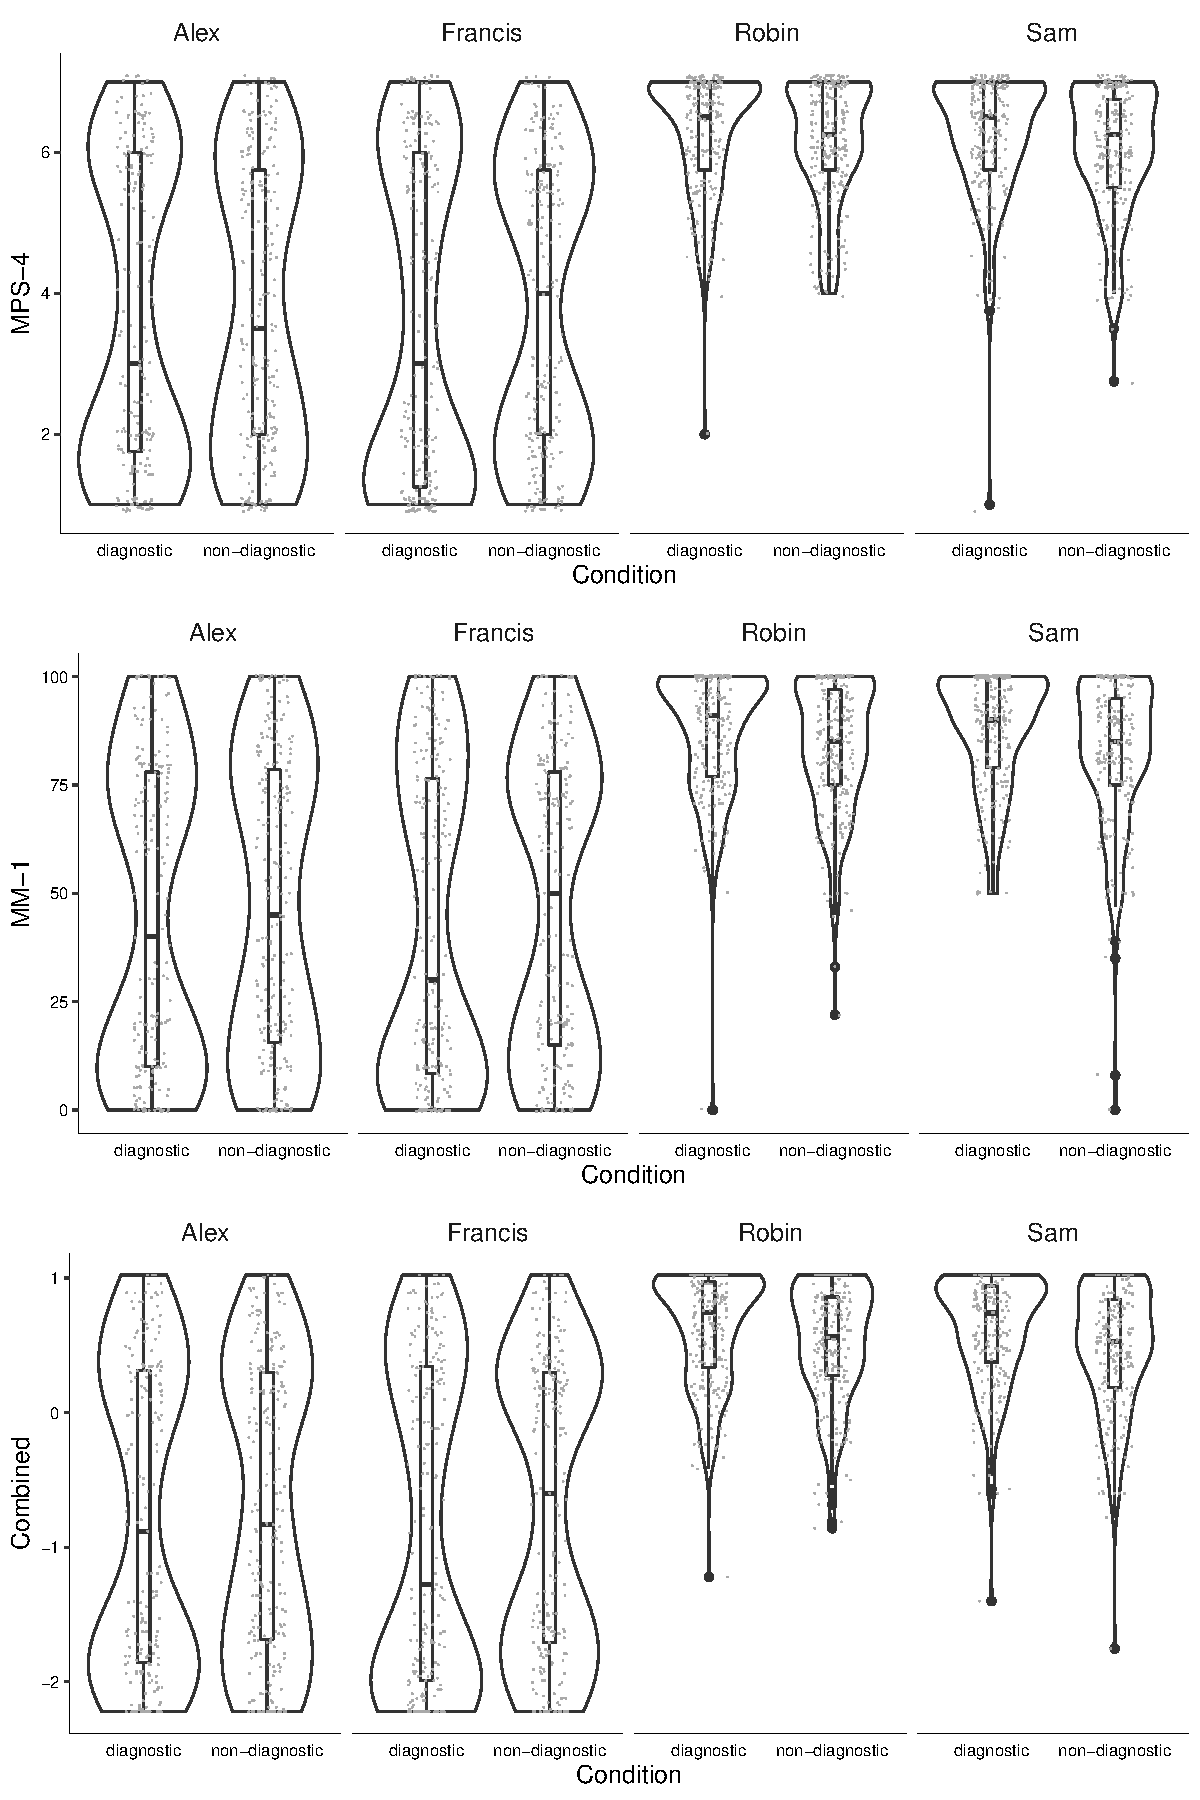
\includegraphics{Supplementary_files/figure-latex/S5allscenariosPlot-1} \caption{Study 5: Differences in moral perception for each description}\label{fig:S5allscenariosPlot}
\end{figure}

For \emph{Sam}, MPS-4 scores were not significantly different in the non-diagnostic condition (\emph{M} = 5.87, \emph{SD} = 0.95), than in the diagnostic condition (\emph{M} = 5.91, \emph{SD} = 0.87), \emph{t}(886.55) = 3.16, \emph{p} = .002, \emph{d} = 0.28; MM-1 ratings were similar in the non-diagnostic condition (\emph{M} = 80.54, \emph{SD} = 14.38), than in the diagnostic condition (\emph{M} = 80.75, \emph{SD} = 13.99), \emph{t}(809.63) = 0.21, \emph{p} = .832, \emph{d} = 0.01. For the combined measure ratings were also similar in the non-diagnostic condition (\emph{M} = -0.05, \emph{SD} = 0.99), than in the diagnostic condition (\emph{M} = -0.01, \emph{SD} = 0.98), \emph{t}(814.30) = 0.55, \emph{p} = .581, \emph{d} = 0.04.

For \emph{Robin}, MPS-4 scores were not significantly different for the non-diagnostic condition (\emph{M} = 6.11, \emph{SD} = 0.86), than in the diagnostic condition (\emph{M} = 6.28, \emph{SD} = 0.83), \emph{t}(448.03) = 2.09, \emph{p} = .037, \emph{d} = 0.20; MM-1 ratings were similar in the non-diagnostic condition (\emph{M} = 83.45, \emph{SD} = 14.86), and in the diagnostic condition (\emph{M} = 87.03, \emph{SD} = 14.14), \emph{t}(448.96) = 2.62, \emph{p} = .009, \emph{d} = 0.25. For the combined measure ratings were also similar in the non-diagnostic condition (\emph{M} = 0.51, \emph{SD} = 0.43), than in the diagnostic condition (\emph{M} = 0.62, \emph{SD} = 0.41), \emph{t}(448.56) = 2.62, \emph{p} = .009, \emph{d} = 0.25.

For \emph{Alex}, MPS-4 scores were not significantly different for the non-diagnostic condition (\emph{M} = 3.78, \emph{SD} = 2.02), than in the diagnostic condition (\emph{M} = 3.67, \emph{SD} = 2.15), \emph{t}(406.27) = -0.55, \emph{p} = .582, \emph{d} = 0.05; MM-1 ratings were similar in the non-diagnostic condition (\emph{M} = 46.75, \emph{SD} = 33.74), than in the diagnostic condition (\emph{M} = 44.80, \emph{SD} = 35.13), \emph{t}(409.65) = -0.58, \emph{p} = .560, \emph{d} = 0.06. For the combined measure ratings were also similar in the non-diagnostic condition (\emph{M} = -0.71, \emph{SD} = 1.06), than in the diagnostic condition (\emph{M} = -0.77, \emph{SD} = 1.13), \emph{t}(406.61) = -0.58, \emph{p} = .562, \emph{d} = 0.06.

For \emph{Francis}, MPS-4 scores were not significantly different for the non-diagnostic condition (\emph{M} = 3.84, \emph{SD} = 2.05), than in the diagnostic condition (\emph{M} = 3.60, \emph{SD} = 2.27), \emph{t}(424.52) = -1.17, \emph{p} = .243, \emph{d} = 0.11; MM-1 ratings were not significantly different in the non-diagnostic condition (\emph{M} = 46.97, \emph{SD} = 34.05), than in the diagnostic condition (\emph{M} = 42.03, \emph{SD} = 35.99), \emph{t}(428.22) = -1.47, \emph{p} = .143, \emph{d} = 0.14. For the combined measure ratings were also similar in the non-diagnostic condition (\emph{M} = -0.69, \emph{SD} = 1.08), and in the diagnostic condition (\emph{M} = -0.84, \emph{SD} = 1.18), \emph{t}(425.90) = -1.35, \emph{p} = .179, \emph{d} = 0.13.

\newpage


\clearpage
\renewcommand{\listfigurename}{Figure captions}

\clearpage
\renewcommand{\listtablename}{Table captions}


\end{document}
